\documentclass{article}[11pt]

\usepackage{natbib}
\usepackage[sc]{mathpazo}
\usepackage[T1]{fontenc}
\usepackage{amsmath}
\usepackage{amsfonts}
\usepackage{amssymb}
\usepackage{graphicx}
\usepackage[onehalfspacing]{setspace}
\usepackage{color}
\usepackage[margin=.75in, tmargin=0.71in, bmargin=0.71in]{geometry}
\usepackage{url}

\usepackage{chngcntr}
\usepackage{appendix}
\usepackage{hyperref}
\usepackage{xcolor}
\usepackage{todonotes}
\usepackage{booktabs}
\usepackage{lscape}
\usepackage{caption}%
\usepackage{bbm}
\usepackage{comment}

\usepackage{blindtext}

\usepackage{longtable}

\usepackage{subcaption}

\usepackage{bookmark}

\usepackage{babel}
\usepackage[autostyle, english = american]{csquotes}
\MakeOuterQuote{"}

% Centered fixed width column type
\usepackage{array}
\newcolumntype{x}[1]{>{\centering\let\newline\\\arraybackslash\hspace{0pt}}m{#1}}

\title{Textual Analysis and Financial Statements}
\author{Isaac Liu with Owen Lin, Chengzheng Xing, and Sean Zhou}

\setlength{\parindent}{0pt}
\setlength{\parskip}{0.5em}

\hypersetup{
    colorlinks=true,
    linkcolor=black,
    filecolor=black,      
    urlcolor=blue,
    citecolor=black
}

% stattotex commands
\newcommand{\avgCompanyMentions}{97.78}
\renewcommand{\avgCompanyMentions}{98.66}
\renewcommand{\avgCompanyMentions}{98.66}


\newcommand{\noCallsWithNonSelfMentions}{1884}
\newcommand{\shareCallsWithNonSelfMentions}{34.2\%}
\renewcommand{\noCallsWithNonSelfMentions}{1884}
\renewcommand{\shareCallsWithNonSelfMentions}{34.2\%}
\renewcommand{\noCallsWithNonSelfMentions}{1884}
\renewcommand{\shareCallsWithNonSelfMentions}{34.2\%}
\renewcommand{\noCallsWithNonSelfMentions}{1884}
\renewcommand{\shareCallsWithNonSelfMentions}{34.2\%}
\renewcommand{\noCallsWithNonSelfMentions}{1884}
\renewcommand{\shareCallsWithNonSelfMentions}{34.2\%}
\renewcommand{\noCallsWithNonSelfMentions}{1884}
\renewcommand{\shareCallsWithNonSelfMentions}{34.2\%}
\renewcommand{\noCallsWithNonSelfMentions}{1884}
\renewcommand{\shareCallsWithNonSelfMentions}{34.2\%}
\renewcommand{\noCallsWithNonSelfMentions}{1,884}
\renewcommand{\noCallsWithNonSelfMentions}{1884}
\renewcommand{\shareCallsWithNonSelfMentions}{34.2\%}
\renewcommand{\noCallsWithNonSelfMentions}{1,884}
\renewcommand{\shareCallsWithNonSelfMentions}{34.2\%}
\renewcommand{\noCallsWithNonSelfMentions}{1,884}
\renewcommand{\shareCallsWithNonSelfMentions}{34.2\%}
\renewcommand{\noCallsWithNonSelfMentions}{1,884}
\renewcommand{\shareCallsWithNonSelfMentions}{34.2\%}


\newcommand{\numQuarters}{4724}
\newcommand{\numCompanies}{387}
\renewcommand{\numQuarters}{4724}
\renewcommand{\numCompanies}{387}
\renewcommand{\numQuarters}{4724}
\renewcommand{\numCompanies}{387}
\renewcommand{\numQuarters}{4724}
\renewcommand{\numCompanies}{387}
\renewcommand{\numQuarters}{4724}
\renewcommand{\numCompanies}{387}
\renewcommand{\numQuarters}{4724}
\renewcommand{\numCompanies}{387}
\renewcommand{\numQuarters}{4724}
\renewcommand{\numCompanies}{387}
\renewcommand{\numQuarters}{4724}
\renewcommand{\numCompanies}{387}
\renewcommand{\numQuarters}{4724}
\renewcommand{\numCompanies}{387}
\renewcommand{\numQuarters}{4724}
\renewcommand{\numCompanies}{387}
\renewcommand{\numQuarters}{4724}
\renewcommand{\numCompanies}{387}
\renewcommand{\numQuarters}{4724}
\renewcommand{\numCompanies}{387}
\renewcommand{\numQuarters}{4724}
\renewcommand{\numCompanies}{387}
\renewcommand{\numQuarters}{4724}
\renewcommand{\numCompanies}{387}
\renewcommand{\numQuarters}{4724}
\renewcommand{\numCompanies}{387}
\renewcommand{\numQuarters}{4,724}
\renewcommand{\numCompanies}{387}
\renewcommand{\numQuarters}{4,724}
\renewcommand{\numCompanies}{387}
\renewcommand{\numQuarters}{4,724}
\renewcommand{\numCompanies}{387}

\newcommand{\avgCallLength}{8,776.18}
\renewcommand{\avgCallLength}{8,754.25}
\renewcommand{\avgCallLength}{8,754.25}
\renewcommand{\avgCallLength}{8,759.68}
\renewcommand{\avgCallLength}{8,759.68}


\newcommand{\shareNotChanges}{0.9358594411515665}
\renewcommand{\shareNotChanges}{0.9358594411515665}
\renewcommand{\shareNotChanges}{0.9358594411515665}
\renewcommand{\shareNotChanges}{93.59\%}
\renewcommand{\shareNotChanges}{93.59\%}
\renewcommand{\shareNotChanges}{93.59\%}
\renewcommand{\shareNotChanges}{93.59\%}
\renewcommand{\shareNotChanges}{94.66\%}
\renewcommand{\shareNotChanges}{94.66\%}
\renewcommand{\shareNotChanges}{94.66\%}
\renewcommand{\shareNotChanges}{94.66\%}
\renewcommand{\shareNotChanges}{94.66\%}
\renewcommand{\shareNotChanges}{94.66\%}
\renewcommand{\shareNotChanges}{94.66\%}
\renewcommand{\shareNotChanges}{94.66\%}


\begin{document}

	\maketitle

    \section*{Introduction}

    Corporate credit ratings represent professional estimations of the default risk carried by company debt. These ratings represent critical information for investors - not just institutional investors and financially sophisticated bondholders, but also stockholders, who may be wiped out completely in the event of bankruptcy. Analyzing ways to predict ratings can offer substantial value to a variety of stakeholders. Predictive models may be useful for investors without access to data, companies or potential lenders that seek information about influential factors,\footnote{There is evidence suggesting financial factors and projections have a causal impact on ratings and are not manipulated by companies in response to forecasted rating changes \citep{he_impact_2018}.} and by any parties seeking interpolated ratings for companies that do not have them.

    In this project, we seek to fully leverage the text of earnings calls, along with traditional financial measures and variables, to improve predictions of corporate credit ratings for any given company and quarter and better understand the importance of various influences.\footnote{Though much literature has focused on financial statements and reports and credit ratings (as just one example, see \cite{makwana_understanding_2022}), our paper takes a relatively underexplored approach, instead incorporating earnings call transcripts. We believe calls offer a richer picture of a firm's financial prospects because they include two-way conversation between company management and financial analysts in form of a Q and A section. This section incorporates the broader beliefs and concerns of the financial community into our predictions. Additionally, in contrast to financial statements, which must be (noisily) parsed to identify sections relevant to management analysis, earnings calls provide more directly valuable and readily available information.} Features capturing call readability, transparency, and engagement join pre-trained language model representations of sentiment \citep{araci_finbert_2019} and traditional tabular variables as inputs to a variety of supervised machine learning techniques for classification from logistic regression to tree-based methods. We also make use of advances in the study of graph neural networks to model linkages between firms implied by mentions in calls. \citep{das_credit_2023}

    To the best of our knowledge, the closest prior work to ours is \cite{donovan_measuring_2021}, which leverages the textual content of earnings calls and financial statements to predict credit events such as bankruptcies, interest spread changes, and rating downgrades. Unigram and bigram word frequencies were used with the supervised machine learning techniques of Support Vector Regression, Latent Dirichlet Allocation, and Random Forests. The coefficient on a constructed textual measure of credit risk was found to be significant up the 1\% level. In contrast to this approach, we focus on predicting the credit ratings themselves, and integrate more recent techniques such as neural language models and a wider variety of algorithms for classification.

    \section*{Data and Exploratory Data Analysis}

    We combine a wide variety of data sources to support our predictions of credit ratings - merging rating data with company earnings calls, financial statement variables, and industry sector. In our combined dataset, each observation represents a fixed quarter date (1/1, 4/1, 7/1, 10/1) for a company, with the company's most recent credit rating, earnings call and associated financial statement variables, and sector attached. An example of many of the variables for a company by fixed quarter date can be found in Appendix Section \ref{sec:one-obs-final-data}.

    Our scope of interest is publicly traded companies from 2010-2016 (a limitation due to the availability of credit rating data) - the distribution of call year and quarters can be found in Appendix Figure \ref{fig:obs-by-quarter-year}. To ensure comparability, we drop items missing any predictor variable, as well as some companies with only a few (3 or less) quarters. We identified one bankruptcy in our data - Peabody Energy on April 13, 2016 - and on further investigation, removed some quarters with incorrect ratings. In all, we have \numQuarters \space quarters for \numCompanies \space unique companies.

    \subsection*{Credit Ratings}

    We make use of long-term credit rating issuances from S and P Rating Services, provided from a combination of two credit rating datasets downloaded in CSV and Excel format from Kaggle \citep{gewerc_corporate_2020,makwana_corporate_2022}. Each issuance can be a change in rating (upgrade, downgrade) or reaffirmation - they occur at ad-hoc intervals. We reshape these rating issuances to a dataset of ratings for each company on each fixed quarter date by creating a rating end date variable that is the date of the next issuance or end of data, and joining a list of the fixed quarter dates on the condition that the fixed quarter date is between the issuance date and the end date.

    POTENTIALLY MOVE ALL DATA CLEANING STEPS TO APPENDIX.

    Figure \ref{fig:credit-ratings} shows the distribution of rating grades used in our final dataset. Finer grades (AA+, CCC-, etc.) are sometimes assigned by agencies, but these grades were converted by dropping the +/- for this project. Ratings of BBB and above are considered investment grade - these bonds carry empirical one-year default rates of 0 to 1\%. Ratings below that are classified as junk, with default rates from 1 to 30, 40, or even 50\% for some years \citep{s_and_p_global_ratings_s_2024}. Most company-quarters have ratings around the BBB threshold, with very few cases on the extreme ends of the spectrum. Ratings also tend to be constant over time. Relative to the previous fixed quarter date, \shareNotChanges \space of ratings remain the same. Rating on the previous fixed quarter date can thus be an extremely strong predictor.

    \begin{figure*}
        \caption{Credit Ratings}
        \begin{subfigure}[h]{0.4925\textwidth}
            \centering
            \subcaption{Distribution}
            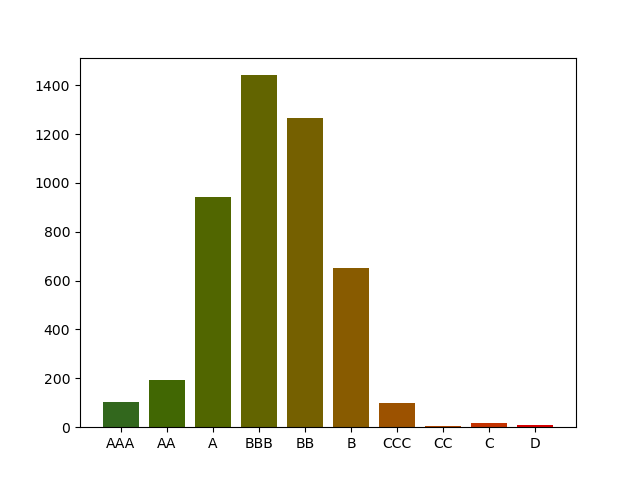
\includegraphics[width=0.95\hsize]{../Output/All Data EDA/Tabular EDA/Distribution of Rating Issuances_no_title.png}
        \end{subfigure}
        %\hfill
        \begin{subfigure}[h]{0.4925\textwidth}
            \centering
            \subcaption{Change Between Fixed Quarter Dates}
            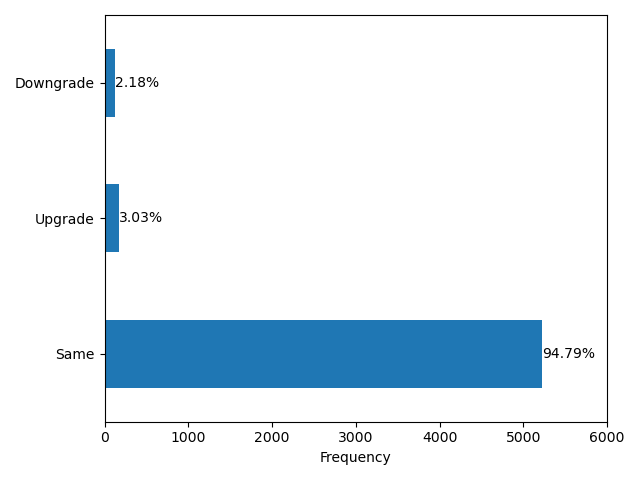
\includegraphics[width=0.95\hsize]{../Output/All Data EDA/Tabular EDA/Change_Short_no_title.png}
        \end{subfigure}
        \hfill
        \label{fig:credit-ratings}
    \end{figure*}

    \subsection*{Earnings Calls}

    Our earnings call data comes from the Financial Modelling Prep API \citep{financial_modeling_prep_financial_2024}, a trusted source widely used in industry. We remove all calls that happened more than 250 days prior and after the first day of the year and quarter they are supposed to discuss the results from, as well as calls for companies that provide them on an annual, rather than quarterly basis. Including both prepared remarks and analyst Q and A sessions, the overall average call length in our final data stands at \avgCallLength \space words.

    \subsection*{Financial Statements}

    Our financial statement variables are also retrieved using the Financial Modelling Prep API. We make use of items from company balance sheets, cash flow statements, and income statements, as well as company market capitalization. We also calculated and included a wide variety of ratios and levels of variables. (for a list, see variables in Table \ref{tab:financial_summary_statistics})
    
    To prepare the data, we limit our observations to items reported in USD, check for and correct values off by a factor of 1,000 as a result of parsing,\footnote{If the last few digits are 000.00 and the item is above or below the 2.5\% and 97.5\% quantile, we divide by 1,000.} and check some accounting identities in \cite{das_credit_2023},\footnote{We check total liabilities are greated than current liabilities, total assets are greater than total current assets, and net sales (revenue) is greated than EBIT. We originally also checked that total assets were greater than or equal to total equity + retained earnings + total liabilities, but this proved to be too restrictive.} setting failing variables to missing. We also discard observations where statement filing dates do not agree between the three types of statements, where the filing date falls outside of the fixed quarter matched on via earnings call date, and where the filing date is more than 45 days after the earnings call date.

    \begin{figure*}
        \caption{Altman Z-Score}
        \begin{subfigure}[h]{0.4925\textwidth}
            \centering
            \subcaption{Distribution}
            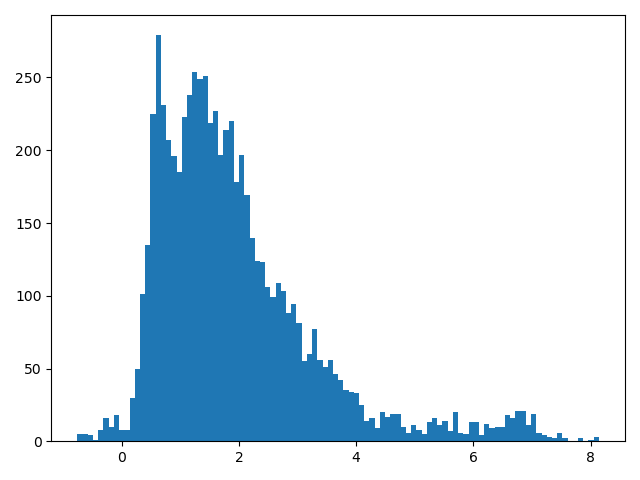
\includegraphics[width=0.95\hsize]{../Output/All Data EDA/Tabular EDA/altman_z_score_all_data_no_title.png}
        \end{subfigure}
        %\hfill
        \begin{subfigure}[h]{0.4925\textwidth}
            \centering
            \subcaption{Average by Rating}
            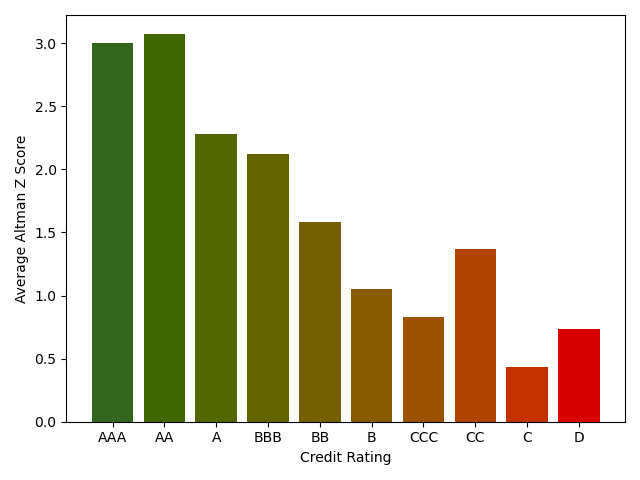
\includegraphics[width=0.95\hsize]{../Output/All Data EDA/Tabular EDA/mean_altman_Z_by_credit_rating_no_title.png}
        \end{subfigure}
        \hfill
        \label{fig:altman-z-score}
    \end{figure*}

    In some of our models, we make use of Altman's Z-score, a traditional measure of bankruptcy risk that accounts for company earnings, equity, and assets and liabilities \citep{altman_financial_1968} (for details on the construction of the score, see Appendix section \ref{sec:altman-z-score}). Figure \ref{fig:altman-z-score} shows the distribution of Z-scores in our dataset. Traditionally, values above 3.0 have been considered safe, while those below 1.8 are considered to have a high chance of bankruptcy. The average scores for each rating in our data seem to align well with this interpretation, with high scores being associated with higher ratings in a linear manner. Aside from a few quirks on the ends of the rating spectrum (where not many companies and ratings are available), Z-Score is likely to be highly useful as a predictor.
      
    \subsection*{Sector}

    The GCIS industry classification standard divides companies into 11 major industry sectors \citep{s_and_p_gics_2024}.\footnote{There are finer groupings as well, but this data was not easily obtainable for our project.} It is widely used in the financial community, and was developed in part by S and P, the same company responsible for our credit ratings. We obtained classifications from Kaggle in CSV format \citep{kozlov_us_2022} and supplemented them with manual lookup. Figure \ref{fig:firms-by-sector} shows the sectoral imbalance present in our data, with a large share of firms in consumer, industrial, and technology sectors. However, when we quantize ratings and compute average values by sector, we do not see large differences, suggesting our results still may provide some generalizability. Though it is not yet clear that sector provides enough useful variation in rating to be a useful predictor, we still include it in our models, particularly as it may improve models including interactions (such as tree-based methods).

    \begin{figure*}
        \caption{Sector}
        \begin{subfigure}[h]{0.4925\textwidth}
            \centering
            \subcaption{Firms by Sector}
            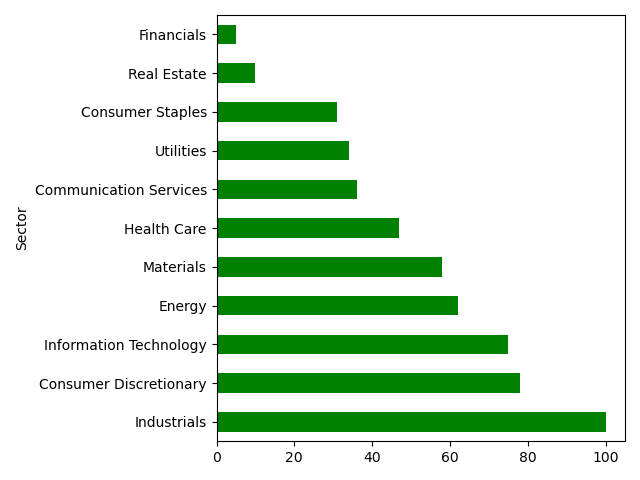
\includegraphics[width=0.95\hsize]{../Output/All Data EDA/Tabular EDA/all_data_fixed_quarter_dates_firms_by_sector_no_title.png}
        \end{subfigure}
        %\hfill
        \begin{subfigure}[h]{0.4925\textwidth}
            \centering
            \subcaption{Average Rating by Sector}
            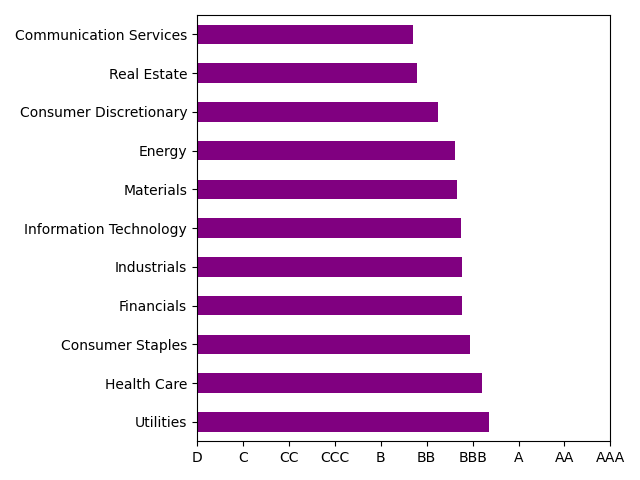
\includegraphics[width=0.95\hsize]{../Output/All Data EDA/Tabular EDA/all_data_fixed_quarter_dates_average_credit_rating_by_sector_no_title.png}
        \end{subfigure}
        \hfill
        \label{fig:firms-by-sector}
    \end{figure*}

    \section*{NLP Features}

    We make use of techniques from Natural Language Processing (NLP) to create features to capture the transparency of discussion, level of engagement, and overall sentiment of calls.

    \begin{itemize}
        \item Numeric Transparency - Ratio of numbers to words in the word-tokenized call
        \item Readability - We construct the Gunning-Fog grade-level readability score \citep{gunning_technique_1952} as 
        \begin{equation*}
            0.4 \times (\frac{\text{Words}}{\text{Sentences}} + 100 \times \frac{\text{3+ Syllable Words}}{\text{Words}})
        \end{equation*}
        \item Word Count
        \item Number of Questions - Count of question marks - Normalized by call length/word count
        \item Tone - Following \cite{price_earnings_2012}, we use the Harvard dictionary to count words falling in various categories (Positive, Negative, Active, Passive, etc.). Then we construct tone using the first principal component of the matrix with each call as a row and each column as one of the following:
        \begin{equation*}
            \frac{\text{Positive}}{\text{Negative}}, \frac{\text{Active}}{\text{Passive}}, \frac{\text{Strong}}{\text{Weak}}, \frac{\text{Overstated}}{\text{Understated}}
        \end{equation*}
        \item FinBERT Positivity Score - \footnote{We originally considered directly incorporating FinBERT embeddings into our models, or creating an end-to-end classifier making use of a BERT model. Our calls, however, are too long for readily available transformer embeddings or models to efficiently and effectively represent.}
    \end{itemize}

    Examples for readability and tone can be found in Appendix Section \ref{sec:nlp-examples}.

    We removed observations with outliers for these features, produced, for example, as a result of zeroes or low values in denominators.
    
    The distribution of each NLP feature by rating is shown in Figure \ref{fig:dist-nlp-by-rating} below. Lower quality companies seem to provide more numbers with less commentary and also have less readable calls (higher Gunning-Fog grade level). It appears to be the case that higher quality companies tend to have longer calls. Though somewhat noisy, our FinBERT positivity score does seem to correlate with higher ratings.

    \begin{figure}[h!]
		\centering
        \caption{Distribution of NLP Features by Rating}
        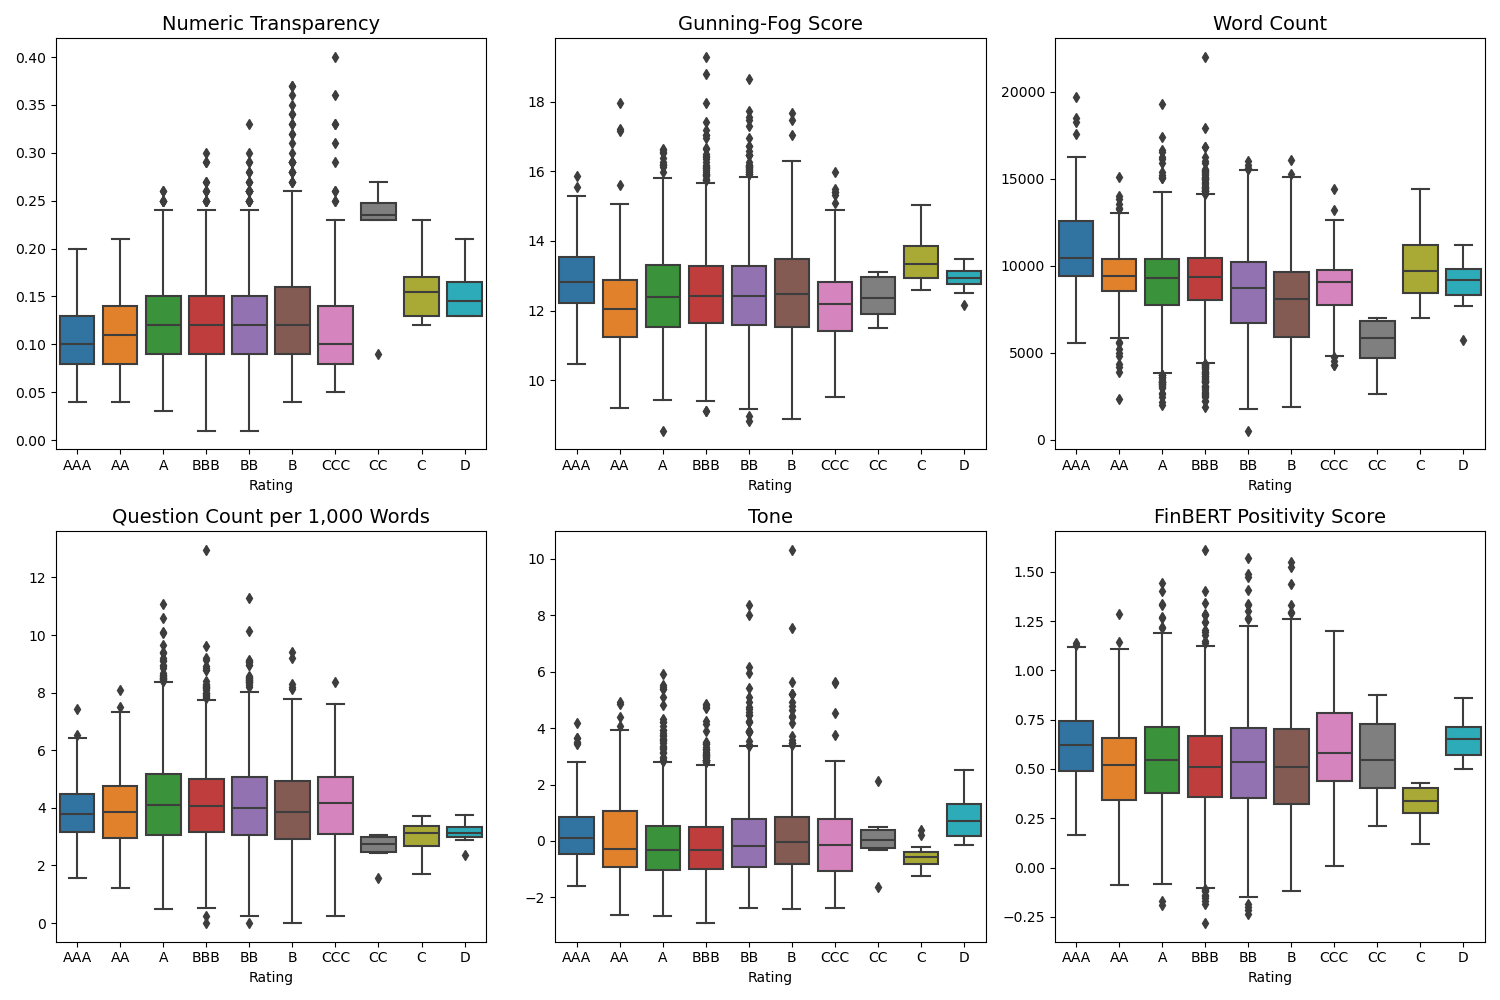
\includegraphics[width=0.6\linewidth,keepaspectratio=true]{../Output/NLP/hist_by_rating.png}
        \label{fig:dist-nlp-by-rating}
	\end{figure}

    \section*{Network of Firms}

    In addition to our standard NLP features, which already capture a rich representation of calls, we also created a network graph representing the connections between firms based on mentions within calls. We deployed transformer-based Named-Entity Recognition (NER) \citep{spacy_spacy_2024} to identify company names in the text, then matched these names to standardized versions. An interative visualization of our entire network of firms (aggregating mentions up from the call level - where we also have a network) can be found at \url{https://sites.google.com/view/isaac-liu/company-mentions-network}, and a ~50\% sample of nodes (faster load time) can be found at \url{https://sites.google.com/view/isaac-liu/co-mentions-50-node-sample}.

    \section*{Modelling}

    Our overall model architecture is of the form

    \begin{equation*}
        \text{Predicted Credit Rating} = f(\text{Altman-Z}, \text{Financial Variables}, \text{Sector}, \text{Previous Rating}, \text{NLP Features})
    \end{equation*}

    We performed an 80-20 train-test split on our data, and used 5-fold cross validation to inform our hyperparameter tuning for the Logistic Regression and XGBoost models.

    \subsection*{Logistic Regression}

    Table \ref{tab:logistic-regression-model-comparison} shows prediction statistics for our initial set of classifiers - simple and interpretable logistic regression models aiming to predict ratings. For these models, we do not include the rating on the previous fixed quarter date (for those results, see Appendix Section \ref{sec:include-previous-rating}). For predicting changes in rating, see Appendix Section \ref{sec:change-prediction}.
    
    \begin{table*}[h!]
        \centering
        \caption{Logistic Regression Model Comparison}
        \footnotesize
\begin{tabular}{ccc}
\toprule
Model/Baseline & Accuracy & Share $\le$ 1 Rating From Actual \\
\midrule
Altman's Z & 0.1923 & 0.4633 \\
Financial Variables and Sector & 0.6225 & 0.9186 \\
Financial Variables, Sector, and NLP Features & 0.6333 & 0.9267 \\
Most Common Class Baseline & 0.3247 &  \\
\bottomrule
\end{tabular}

\normalsize
        \label{tab:logistic-regression-model-comparison}
    \end{table*}

    Altman's Z-Score alone performs poorly - worse than simply assuming each rating belonged to the most common class. Substantial improvement can be attained by adding financial variables (for a list, see items marked as Variable Type ``Additional Ratios'', ``Financial Statements'', and ``'' in Table \ref{tab:numeric_summary_statistics}) as well as sector, and a slight further improvement by adding our NLP features - though this second improvement is not statistically significant. These models including financial variables very frequently bring the predicted rating 1 rating or less away from the actual.

    NOTE MCNEMAR?

    The left side of Table \ref{tab:logistic-most-complex-classification-report-and-permutation-importance} shows that our most complex model generally performs well across all classes, with only a few problems when predicting minority classes. %This is in large part due to our use of balanced class weighting to handle rare classes. We performed grid search 5-fold cross validation to inform our use of these weights. We also found via grid search that an Elastic Net penalty (which collapses to entirely a LASSO penalty) with a slight amount of regularization (C) effectively handles the large number of variables present in our data (for details, see Appendix Section \ref{sec:most-complex-model-additional-details}). 
    
    The right side of Table \ref{tab:logistic-most-complex-classification-report-and-permutation-importance} shows the 15 most important individual features as determined by the average drop in test accuracy when the feature is permuted 1,000 times. Financial features appear to be the most important, with some contributions from our NLP features considering tone and word count.

    RANK NLP FEATURES?

    \begin{table*}[h!]
        \centering
        \caption{Classification Report and Permutation Importance - Most Complex Logistic Regression Model}
        \begin{minipage}[c]{0.45\linewidth}
            \centering
            %\caption{\footnotesize Classification Report - Most Complex Model} 
            \footnotesize
\begin{tabular}{ccccc}
\toprule
Rating & Precision & Recall & F1-Score & Support \\
\midrule
AAA & 0.8261 & 0.7917 & 0.8085 & 24 \\
AA & 0.6316 & 0.6923 & 0.6606 & 52 \\
A & 0.5874 & 0.6298 & 0.6079 & 208 \\
BBB & 0.6909 & 0.6281 & 0.6580 & 363 \\
BB & 0.6275 & 0.5458 & 0.5838 & 284 \\
B & 0.5864 & 0.7273 & 0.6493 & 154 \\
CCC & 0.5556 & 0.7692 & 0.6452 & 26 \\
CC & 0.3333 & 1.0000 & 0.5000 & 2 \\
C & 1.0000 & 1.0000 & 1.0000 & 4 \\
D & 1.0000 & 1.0000 & 1.0000 & 1 \\
\bottomrule
\end{tabular}

\normalsize
            %\label{tab:most-complex-classification-report}
        \end{minipage}
        \begin{minipage}[c]{0.45\linewidth}
            \centering
            %\caption{\footnotesize Permutation Importance - Most Complex Model} 
            \tiny
\begin{tabular}{ccc}
\toprule
Permuted Feature & Mean Accuracy Drop & Standard Deviation \\
\midrule
Ratio E & 0.070625 & 0.009156 \\
Passive Tone & 0.056786 & 0.007741 \\
Sector: Utilities & 0.043208 & 0.005661 \\
Interest Expense & 0.043019 & 0.007802 \\
Ratio D & 0.041765 & 0.007607 \\
Ratio C & 0.040578 & 0.008042 \\
Depreciation and Amortization (Income Statement) & 0.038593 & 0.007163 \\
Net Receivables & 0.036435 & 0.007130 \\
Word Count & 0.035743 & 0.007747 \\
Long-Term Debt & 0.035463 & 0.007198 \\
Market Capitalization & 0.031103 & 0.006867 \\
Goodwill and Intangible Assets & 0.030084 & 0.007430 \\
Gross Profit & 0.027059 & 0.006837 \\
Total Debt & 0.026485 & 0.007413 \\
Net Debt & 0.025156 & 0.007661 \\
\bottomrule
\end{tabular}

\normalsize
            %\label{tab:most-complex-permutation-importance}
        \end{minipage}
        \label{tab:logistic-most-complex-classification-report-and-permutation-importance}
    \end{table*}

    We are also able to inspect the coefficients of our logistic regression model to see if their direction aligns with our intuition concerning the impact of individual features.

    \subsubsection*{XGBoost}

    In Table \ref{tab:xgboost-model-comparison}, we used the popular gradient boosting algorithm XGBoost to predict ratings, finding significant success. With the ability to model complex interactions between variables, we are able to attain substantially higher accuracy when including financial variables, and NLP features provide a statistically significant additional benefit. At around 90\% accuracy, our best model attains a level of performance slightly exceeding that in \cite{das_credit_2023}, with the substantially harder prediction task of predicting from among 10 different ratings (rather than a binary investment grade versus junk classification), and without the affordances of a graph neural network or more complex ensembling. Our model is near perfect in placing ratings within a very close neighborhood of their actual values.

    \begin{table*}[h!]
        \centering
        \caption{XGBoost Model Comparison}
        \footnotesize
\begin{tabular}{ccc}
\toprule
Model/Baseline & Accuracy & Share $\le$ 1 Rating From Actual \\
\midrule
Altman's Z & 0.3855 & 0.7657 \\
Financial Variables and Sector & 0.7630 & 0.9597 \\
Financial Variables, Sector, and NLP Features & 0.9034 & 0.9857 \\
Most Common Class Baseline & 0.3247 &  \\
\bottomrule
\end{tabular}

\normalsize
        \label{tab:xgboost-model-comparison}
    \end{table*}

    Table \ref{tab:xgboost-most-complex-classification-report-and-permutation-importance} demonstrates that this strong performance by our most complex model is consistent across all classes. Financial features appear to be the most important individual variables, though NLP features do also perform well in aggregate. Relative to prior work, our addition of far more financial factors, in combination with complex and transformer-based NLP features, in our large dataset, appears to greatly improve performance.

    % Discuss grid search

    \begin{table*}[h!]
        \centering
        \caption{Classification Report and Permutation Importance - Most Complex XGBoost Model}
        \begin{minipage}[c]{0.45\linewidth}
            \centering
            %\caption{\footnotesize Classification Report - Most Complex Model} 
            \footnotesize
\begin{tabular}{ccccc}
\toprule
Rating & Precision & Recall & F1-Score & Support \\
\midrule
A & 0.8447 & 0.8894 & 0.8665 & 208 \\
AA & 0.8824 & 0.5769 & 0.6977 & 52 \\
AAA & 0.9048 & 0.7917 & 0.8444 & 24 \\
B & 0.9272 & 0.9091 & 0.9180 & 154 \\
BB & 0.9357 & 0.9225 & 0.9291 & 284 \\
BBB & 0.9129 & 0.9532 & 0.9326 & 363 \\
C & 1.0000 & 1.0000 & 1.0000 & 4 \\
CC & 1.0000 & 0.5000 & 0.6667 & 2 \\
CCC & 0.7857 & 0.8462 & 0.8148 & 26 \\
D & 1.0000 & 1.0000 & 1.0000 & 1 \\
\bottomrule
\end{tabular}

\normalsize
            %\label{tab:most-complex-classification-report}
        \end{minipage}
        \begin{minipage}[c]{0.45\linewidth}
            \centering
            %\caption{\footnotesize Permutation Importance - Most Complex Model} 
            \tiny
\begin{tabular}{ccc}
\toprule
Permuted Feature & Mean Accuracy Drop & Standard Deviation \\
\midrule
Retained Earnings & 0.043819 & 0.005761 \\
Market Capitalization & 0.035169 & 0.005735 \\
Dividends Paid & 0.021455 & 0.004481 \\
Debt Ratio & 0.009987 & 0.003413 \\
Common Stock & 0.009693 & 0.002248 \\
Ratio E & 0.009535 & 0.003463 \\
Other Total Stockholders' Equity & 0.009288 & 0.003028 \\
Total Current Liabilities & 0.006888 & 0.002785 \\
Inventory (Balance Sheet) & 0.006802 & 0.002994 \\
Total Current Assets & 0.006684 & 0.003243 \\
Selling General and Administrative Expenses & 0.006031 & 0.002395 \\
Interest Expense & 0.005973 & 0.002740 \\
Net Property Plant Equipment & 0.005729 & 0.001915 \\
Ratio C & 0.005677 & 0.002476 \\
Total Non-Current Assets & 0.005589 & 0.003420 \\
\bottomrule
\end{tabular}

\normalsize
            %\label{tab:most-complex-permutation-importance}
        \end{minipage}
        \label{tab:xgboost-most-complex-classification-report-and-permutation-importance}
    \end{table*}

    \subsubsection*{Graph Neural Network}

    We make use of the network of company mentions within earnings calls to train an end-to-end graph neural network for classification. Graph Neural Networks construct powerful representations of nodes/entities in a network of relationships by using message passing to aggregate features from neighboring nodes. In this work, we use a GraphSAGE \citep{hamilton_inductive_2018} Graph Convolutional Network (GCN) implemented via the Deep Graph Library. \citep{deep_graph_library_deep_2024}

    % begin lyx insertion

    A GraphSage GCN is trained across a number of timesteps (here indexed by $r$) which progressively mix information from the embeddings of more and more distant neighbors. Creating these embeddings for a given timestep is a two-step process.

    First, in the AGG step, the embeddings of the node's direct neighbors are aggregated. Using what is referred to as pool or pooling aggregation, for node $h$, with neighborhood $N(i)$, at timestep $r$,

    \[
    h_{N(i)}^{(r)}=max[(\sigma(W_{pool}h_{j}^{(r-1)}+b),\forall j\in N(i)]
    \]

    meaning the neighboring embeddings from the previous timestep are fed through a fully connected neural network (weights $W_{pool}$, bias $b$, ReLU activation $\sigma)$, and then the elementwise maximum across the new neighbor representations is taken as the aggregated vector.

    Next, during the update (or COMBINE) step, we concatenate the representation of our node of interest from the previous timestep with this aggregated vector, then apply another set of weights and activation to get a fully updated node representation.

    \[
    h_{i}^{(r)}=\sigma(W^{(r)}*CONCAT[h_{i}^{(r-1)},h_{N(i)}^{(r)}])
    \]

    Note that in our implementation the update step has no activation $\sigma$.

    The operations for each timestep ultimately represent a layer of the neural network - a SAGEConv layer, of which we have 3. For our classification task, the last of these produces output of size 9 (number of classes) for each node, while we use vectors of size 32 for intermediate $h$ values. The entire process is trained end-to-end with cross entropy loss. We perform weight decay at rate 5e-4 and train for 100 epochs at a learning rate of 0.01.

    % end lyx insertion

    To initialize our network, we form an unweighted and undirected edge connection between nodes of firm by fixed quarters when a mention occurs in either call.

    Because of the general sparsity of mentions, the size of this network and the size of our training and test datasets for this model is substantially limited.

    GRAPH NN EDA

    Only \noCallsWithNonSelfMentions \space (\shareCallsWithNonSelfMentions \space) have mentions of another company. On average, these calls  mention XXX distinct companies.

    TRANSDUCTIVE VERSUS INDUCTIVE

    CONTRAST with Das et al \cite{das_credit_2023} and note usage of mentions and not cosine similarities

    \section*{Conclusion}

    In this paper we demonstrated methods to incorporate the text of earnings call transcripts to improve predictions of corporate credit ratings. Simple logistic regression achieves middling accuracy on the difficult task of rating prediction, which is not signficantly improved by the addition of NLP features. When we implement XGBoost to better account for interactions between variables, however, performance reaches state-of-the-art/near-state-of-the-art levels, with a substantial contribution from NLP features.

    DISCUSS GRAPH NN RESULTS

    Future work may want to incorporate metadata - days since call, dates and time series components, etc.

    \section*{Acknowledgements}

    Special thanks to the UC Berkeley Stats Department Statistical Computing Facility (SCF). Other acknowledgements: Libor Pospisil, Robert Thompson. GitHub Co-Pilot was used for python code generation (mostly for plotting and table creation/parsing).

    \clearpage
    \newpage

    \bibliographystyle{aea}
    \bibliography{Stat-222-Capstone}

    \clearpage
    \newpage

    \appendix

    % Reset and change numbering for figures and tables
    \counterwithin{figure}{section}
    \counterwithin{table}{section}

    \section{Appendix}

    \subsection{Example of One Observation in Final Data}

    \label{sec:one-obs-final-data}

    Figure \ref{fig:one-obs-final-data} shows some variables for Apple Inc. for the fixed quarter date of October 1, 2014. Apple had a strong rating of AA at this time. This was supported, in part, by a relatively high Altman Z-Score. Sentiment and tone were generally positive, numeric transparency indicates there was a relatively high share of words to numbers (boldly indicating more commentary), and word count was around average.

    \begin{figure*}[h]
        \caption{Apple Inc., October 1, 2014}
        \begin{subfigure}[h]{0.4925\textwidth}
            \centering
            \subcaption{Metadata, Rating, and NLP Features}
            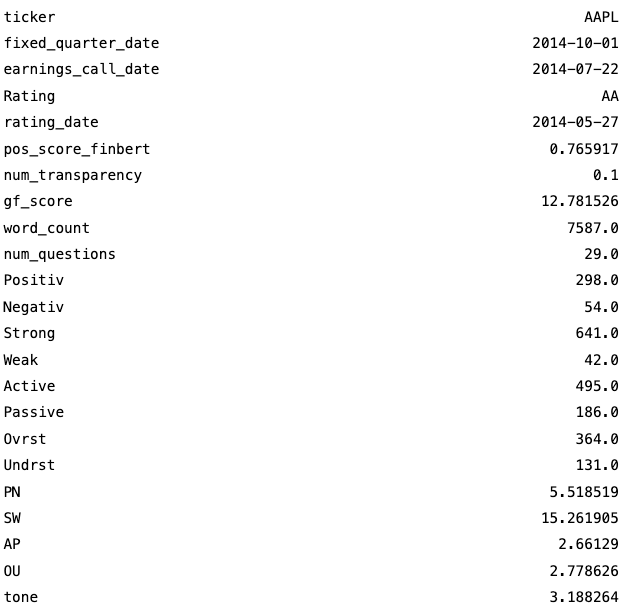
\includegraphics[width=0.95\hsize]{../Output/NLP/aapl nlp.png}
        \end{subfigure}
        %\hfill
        \begin{subfigure}[h]{0.4925\textwidth}
            \centering
            \subcaption{Financial Data}
            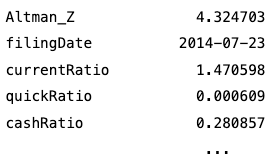
\includegraphics[width=0.5\hsize]{../Output/NLP/aapl fin.png}
        \end{subfigure}
        \hfill
        \label{fig:one-obs-final-data}
    \end{figure*}

    \clearpage
    \newpage

    \subsection{Observations by Quarter and Year}

    Figure \ref{fig:obs-by-quarter-year} demonstrates that the data is temporally unbalanced, with many companies entering the dataset in later years, after they first receive an observable credit rating.

    \begin{figure}[h!]
		\centering
        \caption{Observations by Quarter and Year}
        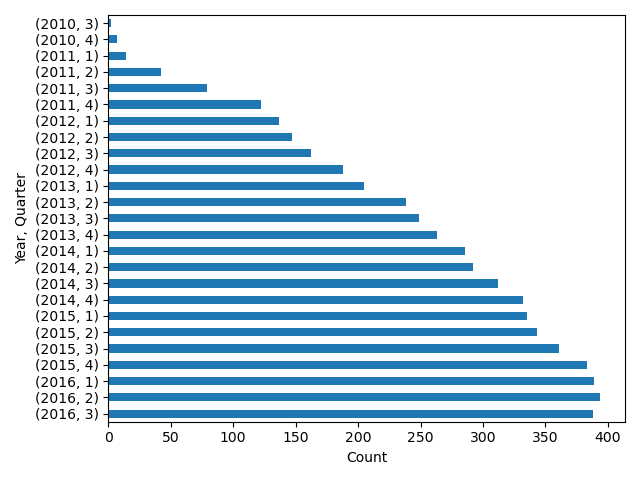
\includegraphics[width=0.6\linewidth,keepaspectratio=true]{../Output/All Data EDA/Tabular EDA/all_data_fixed_quarter_dates_obs_by_year_quarter_no_title.png}
        \label{fig:obs-by-quarter-year}
	\end{figure}
    
    % \clearpage
    % \newpage

    % \subsection{Summary Statistics for Numeric Variables}
    % % Potentially replace with just summary statistics for financial variables

    % Table \ref{tab:numeric_summary_statistics} shows summary statistics for all numeric variables in our dataset. Important numeric and categorical variables are explained in the main text. We also have numerous date variables, which we may use in future predictions.

    % \begin{tabular}{lcccccc}
 & Mean & Minimum & Median & Maximum & Standard Deviation & Variable Type \\
Variable Name &  &  &  &  &  &  \\
Altman's Z Score & 1.88 & -0.91 & 1.58 & 7.56 & 1.30 & Altman's Z Score \\
Accounts Payable (Balance Sheet) & 928,879,944.12 & -237,651,171.00 & 338,150,000.00 & 11,433,000,000.00 & 1,529,128,185.80 & Financial Statements \\
Accounts Payable (Cash Flow Statement) & 4,706,860.62 & -321,769,000.00 & 0.00 & 1,789,652,000.00 & 80,197,009.20 & Financial Statements \\
Accounts Receivables & -10,753,743.96 & -542,000,000.00 & 0.00 & 321,200,000.00 & 90,085,627.31 & Financial Statements \\
Accumulated Other Comprehensive Income (Loss) & -381,975,004.44 & -5,242,000,000.00 & -74,116,000.00 & 431,595,000.00 & 840,987,604.56 & Financial Statements \\
Capital Expenditure & -193,647,213.17 & -1,867,000,000.00 & -59,608,703.91 & 412,700.00 & 314,135,930.83 & Financial Statements \\
Capital Lease Obligations & 28,065,070.59 & 0.00 & 0.00 & 9,056,234,000.00 & 244,927,479.06 & Financial Statements \\
Cash and Cash Equivalents & 852,349,405.25 & 0.00 & 303,118,000.00 & 9,204,000,000.00 & 1,382,415,295.39 & Financial Statements \\
Cash and Short Term Investments & 1,029,007,733.36 & 0.00 & 328,148,000.00 & 15,601,000,000.00 & 1,875,370,693.02 & Financial Statements \\
Cash at Beginning of Period & 857,491,604.07 & -2,556,000.00 & 306,627,000.00 & 9,610,000,000.00 & 1,410,191,719.21 & Financial Statements \\
Cash at End of Period & 866,528,388.67 & -154,400.00 & 307,677,500.00 & 9,743,000,000.00 & 1,425,442,968.51 & Financial Statements \\
Change in Working Capital & -16,292,925.52 & -870,000,000.00 & -1,898,000.00 & 756,000,000.00 & 180,310,959.28 & Financial Statements \\
Common Stock & 332,954,612.87 & -539,800.00 & 3,900,000.00 & 9,817,134,000.00 & 917,174,360.11 & Financial Statements \\
Common Stock Issued & 45,711,557.87 & -3,572,000.00 & 26,500.00 & 906,500,000.00 & 125,660,488.08 & Financial Statements \\
Common Stock Repurchased & -74,290,519.19 & -1,135,000,000.00 & -400,000.00 & 545,656,614.52 & 181,665,328.82 & Financial Statements \\
Cost and Expenses & 2,329,299,450.91 & -2,495,000.00 & 1,109,876,000.00 & 22,496,000,000.00 & 3,409,414,855.37 & Financial Statements \\
Cost of Revenue & 1,630,285,860.24 & -3,094,000.00 & 773,300,000.00 & 16,948,000,000.00 & 2,425,958,117.19 & Financial Statements \\
Debt Repayment & -260,678,959.19 & -3,001,000,000.00 & -35,000,000.00 & 200.00 & 490,067,002.19 & Financial Statements \\
Deferred Income Tax & 5,769,703.18 & -253,000,000.00 & 50,500.00 & 1,850,454,000.00 & 60,203,360.61 & Financial Statements \\
Deferred Revenue & 301,721,276.89 & -116,912,000.00 & 47,100,000.00 & 4,918,100,000.00 & 643,876,051.90 & Financial Statements \\
Depreciation and Amortization (Cash Flow Statement) & 145,689,205.06 & -304,000.00 & 53,427,500.00 & 1,529,000,000.00 & 218,965,861.00 & Financial Statements \\
Depreciation and Amortization (Income Statement) & 142,779,168.92 & -1,550,000.00 & 53,593,000.00 & 1,371,000,000.00 & 210,651,321.79 & Financial Statements \\
Diluted EPS & 0.49 & -156.36 & 0.51 & 49.73 & 3.53 & Financial Statements \\
Dividends Paid & -93,842,514.12 & -1,233,000,000.00 & -21,783,000.00 & 0.00 & 186,830,876.64 & Financial Statements \\
EBITDA & 447,620,359.75 & -66,200,000.00 & 191,346,000.00 & 4,410,000,000.00 & 657,882,497.84 & Financial Statements \\
EBITDA Ratio & 0.20 & -5.77 & 0.18 & 2.16 & 0.23 & Financial Statements \\
EPS & 0.50 & -156.36 & 0.52 & 53.75 & 3.56 & Financial Statements \\
Effect of Foreign Exchange Changes on Cash & -1,647,078.82 & -65,000,000.00 & 0.00 & 52,000,000.00 & 10,955,813.05 & Financial Statements \\
Free Cash Flow & 152,488,089.91 & -541,000,000.00 & 50,350,500.00 & 2,683,000,000.00 & 386,075,408.86 & Financial Statements \\
General and Administrative Expenses & 142,016,375.14 & -2,117,000.00 & 30,257,000.00 & 2,007,000,000.00 & 288,668,731.35 & Financial Statements \\
Goodwill & 1,971,783,101.42 & -202,702,100.00 & 626,536,500.00 & 23,389,000,000.00 & 3,541,028,978.34 & Financial Statements \\
Goodwill and Intangible Assets & 3,143,944,231.55 & -1,618,944,000.00 & 962,312,000.00 & 37,123,000,000.00 & 5,784,596,899.63 & Financial Statements \\
Gross Profit & 872,368,464.63 & -7,195,000.00 & 373,018,500.00 & 9,223,000,000.00 & 1,421,025,818.62 & Financial Statements \\
Gross Profit Ratio & 0.37 & -5.65 & 0.34 & 2.19 & 0.27 & Financial Statements \\
Income Before Tax & 249,496,947.58 & -353,153,000.00 & 89,895,500.00 & 2,951,000,000.00 & 434,495,406.26 & Financial Statements \\
Income Before Tax Ratio & 0.07 & -9.38 & 0.09 & 1.27 & 0.37 & Financial Statements \\
Income Tax Expense & 68,390,107.98 & -119,131,000.00 & 21,775,500.00 & 736,000,000.00 & 121,599,241.07 & Financial Statements \\
Intangible Assets & 869,968,811.22 & -421,000.00 & 173,358,000.00 & 14,110,100,000.00 & 1,855,409,062.61 & Financial Statements \\
Interest Expense & 49,203,706.71 & -16,400,000.00 & 23,385,000.00 & 386,000,000.00 & 65,029,625.22 & Financial Statements \\
Interest Income & 2,335,687.82 & -32,293.00 & 0.00 & 69,000,000.00 & 6,967,205.85 & Financial Statements \\
Inventory (Balance Sheet) & 958,995,636.94 & -19,626,000.00 & 414,950,000.00 & 8,328,000,000.00 & 1,433,396,913.56 & Financial Statements \\
Inventory (Cash Flow Statement) & -10,636,842.51 & -420,000,000.00 & 0.00 & 289,000,000.00 & 70,202,756.90 & Financial Statements \\
Investments in Property, Plants, and Equipment & -194,860,014.81 & -1,921,864,000.00 & -59,719,000.00 & 412,700.00 & 317,067,486.90 & Financial Statements \\
Long-Term Debt & 4,342,642,310.38 & 0.00 & 1,843,812,000.00 & 31,228,000,000.00 & 5,794,340,264.76 & Financial Statements \\
Long-Term Investments & 521,054,256.46 & -490,677,000.00 & 11,203,500.00 & 10,981,000,000.00 & 1,427,052,488.42 & Financial Statements \\
Minority Interest & 96,515,825.94 & -286,000.00 & 1,784,000.00 & 2,316,406,000.00 & 283,036,455.78 & Financial Statements \\
Net Acquisitions & -31,252,849.61 & -805,960,000.00 & 0.00 & 249,000,000.00 & 113,700,319.45 & Financial Statements \\
Net Cash Provided by Operating Activities & 353,695,946.55 & -175,500,000.00 & 142,068,000.00 & 3,870,000,000.00 & 559,577,854.70 & Financial Statements \\
Net Cash Used for Investing Activities & -252,301,738.93 & -2,840,033,000.00 & -69,018,000.00 & 325,900,000.00 & 447,680,994.35 & Financial Statements \\
Net Cash Used or Provided by Financing Activities & -113,094,742.90 & -2,444,000,000.00 & -28,913,000.00 & 1,094,000,000.00 & 398,976,123.98 & Financial Statements \\
Net Change in Cash & 6,986,471.31 & -1,161,000,000.00 & 326,500.00 & 1,401,000,000.00 & 262,805,651.94 & Financial Statements \\
Net Debt & 3,807,913,408.87 & -1,044,500,000.00 & 1,567,100,000.00 & 30,761,000,000.00 & 5,555,751,832.58 & Financial Statements \\
Net Income (Cash Flow Statement) & 186,107,161.79 & -327,000,000.00 & 64,393,500.00 & 2,402,000,000.00 & 338,084,813.74 & Financial Statements \\
Net Income (Income Statement) & 183,234,857.90 & -329,864,000.00 & 64,300,000.00 & 2,340,000,000.00 & 335,149,633.65 & Financial Statements \\
Net Income Ratio & 0.05 & -8.88 & 0.07 & 2.72 & 0.31 & Financial Statements \\
Net Property Plant Equipment & 5,007,874,719.10 & 0.00 & 1,389,082,500.00 & 44,441,000,000.00 & 8,045,435,934.42 & Financial Statements \\
Net Receivables & 1,259,577,298.60 & -4,199,600.00 & 539,100,000.00 & 12,146,000,000.00 & 1,814,088,013.82 & Financial Statements \\
Non-Current Deferred Revenue & 250,512,754.02 & -500,933,000.00 & 0.00 & 5,778,000,000.00 & 727,888,527.14 & Financial Statements \\
Non-Current Deferred Tax Liabilities & 698,746,738.38 & -3,818,507.00 & 133,077,500.00 & 8,306,000,000.00 & 1,425,671,155.54 & Financial Statements \\
Operating Cash Flow & 353,695,946.55 & -175,500,000.00 & 142,068,000.00 & 3,870,000,000.00 & 559,577,854.70 & Financial Statements \\
Operating Expenses & 547,725,941.27 & -13,530,000.00 & 211,937,500.00 & 6,252,000,000.00 & 959,936,714.19 & Financial Statements \\
Operating Income & 298,743,632.43 & -208,377,000.00 & 119,850,000.00 & 3,294,000,000.00 & 476,982,715.49 & Financial Statements \\
Operating Income Ratio & 0.10 & -9.71 & 0.12 & 1.14 & 0.33 & Financial Statements \\
Other Assets & 8,191.33 & -19,834,700.00 & 0.00 & 8,948,000.00 & 468,348.06 & Financial Statements \\
Other Current Assets & 380,708,173.61 & -49,000.00 & 113,056,500.00 & 4,968,950,000.00 & 690,346,469.76 & Financial Statements \\
Other Current Liabilities & 990,758,356.70 & -48,317,000.00 & 322,670,500.00 & 12,137,000,000.00 & 1,870,004,710.84 & Financial Statements \\
Other Expenses & 49,916,440.59 & -64,000,000.00 & 608,500.00 & 16,189,674,590.00 & 363,247,062.24 & Financial Statements \\
Other Financing Activities & 221,463,311.27 & -975,168,999.00 & 8,000,000.00 & 3,297,501,000.00 & 524,943,949.61 & Financial Statements \\
Other Investing Activities & 4,791,113.98 & -448,000,000.00 & 123,500.00 & 3,060,433,659.00 & 97,646,984.87 & Financial Statements \\
Other Liabilities & 111,303.72 & -267,212.00 & 0.00 & 51,076,000.00 & 2,208,107.68 & Financial Statements \\
Other Non-Cash Items & 14,733,647.77 & -1,848,719,007.00 & 1,562,000.00 & 699,000,000.00 & 105,972,613.46 & Financial Statements \\
Other Non-Current Assets & 526,230,472.94 & -75,012,534,818.00 & 154,478,500.00 & 8,037,000,000.00 & 1,892,020,258.31 & Financial Statements \\
Other Non-Current Liabilities & 973,607,594.44 & -286,041,895.00 & 326,195,000.00 & 11,890,564,000.00 & 1,729,729,702.42 & Financial Statements \\
Other Total Stockholders' Equity & 1,058,480,401.28 & -12,393,000,000.00 & 387,440,500.00 & 34,030,400,000.00 & 3,676,996,160.82 & Financial Statements \\
Other Working Capital & 20,095,755.18 & -1,788,851,160.00 & 0.00 & 40,341,689,407.00 & 784,774,785.47 & Financial Statements \\
Preferred Stock & 8,957,412.19 & 0.00 & 0.00 & 401,500,000.00 & 41,741,915.35 & Financial Statements \\
Purchases of Investments & -99,111,435.92 & -11,997,654,000.00 & 0.00 & 81,823,000.00 & 344,843,591.76 & Financial Statements \\
Research and Development Expenses & 24,546,760.47 & -214,000.00 & 0.00 & 893,000,000.00 & 90,083,795.75 & Financial Statements \\
Retained Earnings & 3,629,692,655.97 & -4,839,000,000.00 & 1,274,232,500.00 & 37,899,000,000.00 & 6,497,897,135.46 & Financial Statements \\
Revenue & 2,752,115,994.55 & -4,273,000.00 & 1,283,674,000.00 & 25,420,000,000.00 & 4,046,436,838.80 & Financial Statements \\
Sales and Maturities of Investments & 92,477,266.23 & -9,409,000.00 & 0.00 & 8,936,406,000.00 & 303,356,990.01 & Financial Statements \\
Selling General and Administrative Expenses & 293,844,085.52 & -2,117,000.00 & 114,052,500.00 & 3,333,000,000.00 & 495,298,108.22 & Financial Statements \\
Selling and Marketing Expenses & 25,337,708.44 & -3,003,000.00 & 0.00 & 876,761,000.00 & 98,783,957.01 & Financial Statements \\
Short Term Investments & 171,674,306.11 & -515,000.00 & 0.00 & 6,178,000,000.00 & 570,578,944.19 & Financial Statements \\
Short-Term Debt & 488,398,947.44 & -655,561.00 & 89,034,500.00 & 5,359,000,000.00 & 919,311,633.83 & Financial Statements \\
Stock-Based Compensation & 14,271,901.15 & -36,000,000.00 & 4,956,500.00 & 254,000,000.00 & 30,389,470.84 & Financial Statements \\
Tax Assets & 374,484,728.56 & -2,310,712,000.00 & 45,781,000.00 & 6,535,000,000.00 & 917,009,577.63 & Financial Statements \\
Tax Payable & 60,320,998.32 & -87,400.00 & 2,916,000.00 & 1,183,200,000.00 & 151,310,152.81 & Financial Statements \\
Total Assets & 16,041,516,101.31 & 123,279.00 & 6,776,797,500.00 & 131,556,000,000.00 & 22,888,760,450.42 & Financial Statements \\
Total Current Assets & 3,956,106,957.32 & 35,587.00 & 1,887,586,000.00 & 41,276,000,000.00 & 5,914,890,504.74 & Financial Statements \\
Total Current Liabilities & 2,841,825,102.84 & 12,178.00 & 1,101,173,000.00 & 29,919,000,000.00 & 4,386,480,010.78 & Financial Statements \\
Total Debt & 4,788,891,751.88 & 2,000.00 & 2,037,148,000.00 & 37,124,000,000.00 & 6,477,270,025.47 & Financial Statements \\
Total Equity & 5,025,612,554.17 & -501,467,000.00 & 2,029,718,000.00 & 49,975,000,000.00 & 7,546,463,280.10 & Financial Statements \\
Total Investments & 762,733,616.78 & -334,673,000.00 & 38,129,000.00 & 19,331,000,000.00 & 2,065,926,624.79 & Financial Statements \\
Total Liabilities & 10,144,020,041.90 & 79,283.00 & 4,287,428,500.00 & 87,293,000,000.00 & 14,121,143,146.21 & Financial Statements \\
Total Liabilities and Stockholders' Equity & 16,005,558,652.32 & 123,279.00 & 6,776,797,500.00 & 131,556,000,000.00 & 22,880,811,656.54 & Financial Statements \\
Total Liabilities and Total Equity & 16,005,558,652.32 & 123,279.00 & 6,776,797,500.00 & 131,556,000,000.00 & 22,880,811,656.54 & Financial Statements \\
Total Non-Current Assets & 11,376,619,839.67 & 49,861.00 & 4,137,290,500.00 & 104,263,000,000.00 & 16,727,793,153.36 & Financial Statements \\
Total Non-Current Liabilities & 6,875,270,635.58 & 53,696.00 & 2,800,400,000.00 & 54,300,000,000.00 & 9,789,172,194.03 & Financial Statements \\
Total Other Income Expenses Net & -12,311,364.49 & -503,976,000.00 & -795,000.00 & 286,000,000.00 & 72,409,332.85 & Financial Statements \\
Total Stockholders' Equity & 4,987,566,971.51 & -526,491,000.00 & 2,028,600,000.00 & 49,269,000,000.00 & 7,466,218,430.87 & Financial Statements \\
Weighted Average Shares Outstanding & 361,410,798.65 & 0.00 & 145,598,222.50 & 13,751,391,147.00 & 752,501,668.54 & Financial Statements \\
Weighted Average Shares Outstanding (Diluted) & 322,626,084.79 & 0.00 & 144,583,000.00 & 13,986,214,405.00 & 577,545,825.69 & Financial Statements \\
Market Capitalization & 20,034,247,568.22 & 106,422.00 & 6,348,776,650.00 & 726,320,349,360.00 & 47,265,667,703.74 & Market Capitalization \\
Days Since Call & 58.21 & 0.00 & 61.00 & 91.00 & 13.30 & Metadata \\
First Principal Component of Tone & -0.01 & -2.64 & -0.20 & 25.35 & 1.34 & NLP Feature \\
Gunning-Fog Score & 12.52 & 8.55 & 12.43 & 19.29 & 1.32 & NLP Feature \\
Number of Questions & 36.24 & 0.00 & 35.00 & 107.00 & 16.29 & NLP Feature \\
Numeric Transparency & 0.12 & 0.01 & 0.12 & 0.40 & 0.05 & NLP Feature \\
Postitivity Score & 0.19 & -0.20 & 0.18 & 0.65 & 0.10 & NLP Feature \\
Readability & 12.52 & 8.55 & 12.43 & 19.29 & 1.32 & NLP Feature \\
Word Count & 8,851.58 & 1,782.00 & 9,077.00 & 22,006.00 & 2,489.13 & NLP Feature \\
Change Since Last Fixed Quarter Date & 0.01 & -2.00 & 0.00 & 2.00 & 0.29 & Predicted - Change \\
\end{tabular}


    \clearpage
    \newpage

    \subsection{Summary Statistics for Financial Variables}

    Table \ref{tab:financial_summary_statistics} shows summary statistics for all numeric variables in our dataset. Other important variables are explained in the main text.

    \tiny
\begin{longtable}{ccccccc}
\caption{Financial Variable Summary Statistics} \label{tab:financial_summary_statistics} \\
\toprule
Variable Name & Mean & Minimum & Median & Maximum & Standard Deviation & Variable Type \\
\midrule
\endfirsthead
\caption[]{Financial Variable Summary Statistics} \\
\toprule
Variable Name & Mean & Minimum & Median & Maximum & Standard Deviation & Variable Type \\
\midrule
\endhead
\midrule
\multicolumn{7}{r}{Continued on next page} \\
\midrule
\endfoot
\bottomrule
\endlastfoot
Cash Per Share & 4.57 & 0.00 & 2.13 & 69.91 & 9.64 & Additional Ratios \\
Cash Ratio & 1.21 & 0.00 & 0.28 & 53.17 & 6.23 & Additional Ratios \\
Current Ratio & 1.93 & 0.35 & 1.58 & 7.93 & 1.33 & Additional Ratios \\
Debt Ratio & 0.35 & 0.00 & 0.32 & 0.94 & 0.19 & Additional Ratios \\
Debt Ratio (Alternative Definition) & 0.65 & 0.28 & 0.64 & 1.22 & 0.17 & Additional Ratios \\
Debt to Equity Ratio & -34.63 & -1,890.41 & 1.70 & 25.40 & 256.02 & Additional Ratios \\
EBIT to Revenue & 0.12 & -0.26 & 0.11 & 0.47 & 0.12 & Additional Ratios \\
Enterprise Value Multiplier & 59.08 & -309.75 & 40.67 & 727.20 & 125.93 & Additional Ratios \\
Equity Multiplier & -22.79 & -1,270.10 & 2.71 & 22.64 & 175.08 & Additional Ratios \\
Free Cash Flow Per Share & 0.57 & -2.98 & 0.39 & 7.70 & 1.52 & Additional Ratios \\
Free Cash Flow to Operating Cash Flow & 0.72 & -2.42 & 0.66 & 10.98 & 1.86 & Additional Ratios \\
Operating Cash Flow Per Share & 1.48 & -0.98 & 1.04 & 11.82 & 1.92 & Additional Ratios \\
Operating Cash Flow to Sales & 0.16 & -0.15 & 0.14 & 0.64 & 0.15 & Additional Ratios \\
Quick Ratio & 1.36 & 0.00 & 1.15 & 6.12 & 0.98 & Additional Ratios \\
Return on Assets & 0.01 & -0.03 & 0.01 & 0.06 & 0.02 & Additional Ratios \\
Return on Capital Employed & 0.03 & -0.03 & 0.02 & 0.11 & 0.03 & Additional Ratios \\
Return on Equity & 0.01 & -1.32 & 0.03 & 0.78 & 0.25 & Additional Ratios \\
Accounts Payable (Balance Sheet) & 957,290,323.93 & -237,651,171.00 & 356,700,000.00 & 11,433,000,000.00 & 1,551,108,353.02 & Financial Statements \\
Accounts Payable (Cash Flow Statement) & 5,154,565.15 & -321,769,000.00 & 0.00 & 1,789,652,000.00 & 82,110,968.91 & Financial Statements \\
Accounts Receivables & -11,478,236.25 & -544,000,000.00 & 0.00 & 325,000,000.00 & 91,535,961.30 & Financial Statements \\
Accumulated Other Comprehensive Income (Loss) & -404,483,300.22 & -5,290,000,000.00 & -77,514,000.00 & 431,595,000.00 & 874,353,108.41 & Financial Statements \\
Capital Expenditure & -192,514,484.47 & -1,867,000,000.00 & -60,129,000.00 & 412,700.00 & 310,057,440.27 & Financial Statements \\
Capital Lease Obligations & 24,642,498.79 & 0.00 & 0.00 & 9,056,234,000.00 & 228,328,885.18 & Financial Statements \\
Cash and Cash Equivalents & 862,135,865.07 & 0.00 & 333,000,000.00 & 9,223,000,000.00 & 1,366,595,243.17 & Financial Statements \\
Cash and Short Term Investments & 1,060,086,810.64 & 0.00 & 363,008,000.00 & 15,601,000,000.00 & 1,890,682,420.93 & Financial Statements \\
Cash at Beginning of Period & 867,410,489.82 & -2,556,000.00 & 334,000,000.00 & 9,610,000,000.00 & 1,388,834,800.13 & Financial Statements \\
Cash at End of Period & 871,017,693.39 & -154,400.00 & 335,469,000.00 & 9,743,000,000.00 & 1,394,641,397.30 & Financial Statements \\
Change in Working Capital & -17,557,103.20 & -870,000,000.00 & -2,384,000.00 & 753,000,000.00 & 183,788,257.05 & Financial Statements \\
Common Stock & 329,277,684.36 & -539,800.00 & 3,800,000.00 & 9,817,134,000.00 & 925,626,949.20 & Financial Statements \\
Common Stock Issued & 44,672,509.36 & -3,572,000.00 & 43,000.00 & 1,111,490,728.00 & 124,027,450.20 & Financial Statements \\
Common Stock Repurchased & -78,527,033.90 & -2,086,545,366.00 & -773,000.00 & 545,656,614.52 & 188,219,352.34 & Financial Statements \\
Cost and Expenses & 2,317,513,877.07 & -2,495,000.00 & 1,121,064,000.00 & 22,769,000,000.00 & 3,357,899,606.58 & Financial Statements \\
Cost of Revenue & 1,624,233,369.18 & -3,094,000.00 & 787,700,000.00 & 18,303,000,000.00 & 2,405,765,370.43 & Financial Statements \\
Debt Repayment & -247,880,234.24 & -3,001,000,000.00 & -33,400,000.00 & 200.00 & 471,724,050.37 & Financial Statements \\
Deferred Income Tax & 6,154,669.54 & -253,000,000.00 & 64,000.00 & 1,850,454,000.00 & 58,927,713.28 & Financial Statements \\
Deferred Revenue & 310,000,739.66 & -116,912,000.00 & 50,066,000.00 & 4,918,100,000.00 & 642,489,899.31 & Financial Statements \\
Depreciation and Amortization (Cash Flow Statement) & 141,811,048.14 & -675,312.00 & 53,551,000.00 & 1,529,000,000.00 & 210,315,836.18 & Financial Statements \\
Depreciation and Amortization (Income Statement) & 140,571,212.83 & -1,550,000.00 & 54,507,000.00 & 1,371,000,000.00 & 203,167,331.44 & Financial Statements \\
Diluted EPS & 0.51 & -156.36 & 0.51 & 49.73 & 3.31 & Financial Statements \\
Dividends Paid & -91,357,096.76 & -1,233,000,000.00 & -21,054,000.00 & 0.00 & 182,429,714.55 & Financial Statements \\
EBITDA & 444,995,396.82 & -66,200,000.00 & 193,000,000.00 & 4,410,000,000.00 & 644,706,471.62 & Financial Statements \\
EBITDA Ratio & 0.20 & -5.77 & 0.17 & 2.16 & 0.22 & Financial Statements \\
EPS & 0.52 & -156.36 & 0.52 & 53.75 & 3.33 & Financial Statements \\
Effect of Foreign Exchange Changes on Cash & -1,697,085.83 & -65,000,000.00 & 0.00 & 52,000,000.00 & 11,200,007.88 & Financial Statements \\
Free Cash Flow & 156,892,657.81 & -541,000,000.00 & 51,691,000.00 & 2,683,000,000.00 & 389,666,937.19 & Financial Statements \\
General and Administrative Expenses & 153,933,016.99 & -2,738,500.00 & 33,768,000.00 & 2,007,000,000.00 & 303,900,948.38 & Financial Statements \\
Goodwill & 2,009,260,205.06 & -202,702,100.00 & 636,039,000.00 & 23,389,000,000.00 & 3,554,057,246.39 & Financial Statements \\
Goodwill and Intangible Assets & 3,102,882,804.88 & -1,618,944,000.00 & 970,000,000.00 & 37,123,000,000.00 & 5,639,038,312.52 & Financial Statements \\
Gross Profit & 861,821,178.07 & -7,195,000.00 & 378,500,000.00 & 9,223,000,000.00 & 1,365,410,717.45 & Financial Statements \\
Gross Profit Ratio & 0.37 & -5.65 & 0.34 & 2.32 & 0.26 & Financial Statements \\
Income Before Tax & 255,351,974.53 & -353,153,000.00 & 91,900,000.00 & 2,951,000,000.00 & 434,623,029.43 & Financial Statements \\
Income Before Tax Ratio & 0.07 & -9.38 & 0.09 & 2.68 & 0.35 & Financial Statements \\
Income Tax Expense & 69,444,774.33 & -119,131,000.00 & 22,100,000.00 & 736,000,000.00 & 121,681,731.43 & Financial Statements \\
Intangible Assets & 835,940,509.51 & -421,000.00 & 170,197,000.00 & 14,110,100,000.00 & 1,785,542,119.17 & Financial Statements \\
Interest Expense & 46,568,508.69 & -16,400,000.00 & 23,000,000.00 & 386,000,000.00 & 61,712,161.15 & Financial Statements \\
Interest Income & 2,372,725.23 & -62,900.00 & 0.00 & 69,000,000.00 & 6,859,086.75 & Financial Statements \\
Inventory (Balance Sheet) & 933,043,177.40 & -19,626,000.00 & 403,789,000.00 & 8,328,000,000.00 & 1,398,934,358.21 & Financial Statements \\
Inventory (Cash Flow Statement) & -10,302,495.14 & -420,000,000.00 & 0.00 & 289,000,000.00 & 70,374,129.32 & Financial Statements \\
Investments in Property, Plants, and Equipment & -193,897,744.95 & -1,921,864,000.00 & -60,373,000.00 & 412,700.00 & 313,436,441.14 & Financial Statements \\
Long-Term Debt & 4,159,473,460.27 & -651,718.00 & 1,822,139,000.00 & 31,359,000,000.00 & 5,574,538,232.32 & Financial Statements \\
Long-Term Investments & 494,196,440.41 & -490,677,000.00 & 12,449,000.00 & 10,981,000,000.00 & 1,359,571,399.50 & Financial Statements \\
Minority Interest & 90,043,651.07 & -20,252,654.04 & 1,600,000.00 & 2,316,406,000.00 & 268,200,905.93 & Financial Statements \\
Net Acquisitions & -32,878,764.18 & -805,960,000.00 & 0.00 & 249,000,000.00 & 116,107,004.20 & Financial Statements \\
Net Cash Provided by Operating Activities & 352,446,106.81 & -179,404,000.00 & 143,626,000.00 & 3,870,000,000.00 & 545,602,564.63 & Financial Statements \\
Net Cash Used for Investing Activities & -252,575,304.44 & -2,840,033,000.00 & -71,100,000.00 & 325,900,000.00 & 443,647,871.52 & Financial Statements \\
Net Cash Used or Provided by Financing Activities & -114,570,062.00 & -2,444,000,000.00 & -29,157,000.00 & 1,094,000,000.00 & 399,330,481.52 & Financial Statements \\
Net Change in Cash & 3,933,018.18 & -1,161,000,000.00 & 573,000.00 & 1,401,000,000.00 & 269,005,283.68 & Financial Statements \\
Net Debt & 3,597,141,664.59 & -1,044,500,000.00 & 1,508,594,000.00 & 30,761,000,000.00 & 5,338,457,121.62 & Financial Statements \\
Net Income (Cash Flow Statement) & 189,122,176.12 & -327,000,000.00 & 66,190,000.00 & 2,402,000,000.00 & 336,635,167.35 & Financial Statements \\
Net Income (Income Statement) & 185,944,828.27 & -329,864,000.00 & 66,389,000.00 & 2,340,000,000.00 & 330,952,161.49 & Financial Statements \\
Net Income Ratio & 0.05 & -8.88 & 0.07 & 2.72 & 0.29 & Financial Statements \\
Net Property Plant Equipment & 4,931,687,321.78 & 0.00 & 1,389,600,000.00 & 44,441,000,000.00 & 7,885,938,319.99 & Financial Statements \\
Net Receivables & 1,276,905,848.63 & -4,199,600.00 & 570,338,000.00 & 12,116,000,000.00 & 1,776,578,353.43 & Financial Statements \\
Non-Current Deferred Revenue & 248,840,448.23 & -500,933,000.00 & 0.00 & 5,778,000,000.00 & 723,186,467.01 & Financial Statements \\
Non-Current Deferred Tax Liabilities & 702,874,797.74 & -3,818,507.00 & 135,597,000.00 & 8,306,000,000.00 & 1,400,029,509.57 & Financial Statements \\
Operating Cash Flow & 352,446,106.81 & -179,404,000.00 & 143,626,000.00 & 3,870,000,000.00 & 545,602,564.63 & Financial Statements \\
Operating Expenses & 538,189,512.49 & -13,530,000.00 & 221,700,000.00 & 6,252,000,000.00 & 918,426,909.60 & Financial Statements \\
Operating Income & 302,231,079.76 & -208,377,000.00 & 122,000,000.00 & 3,294,000,000.00 & 475,077,278.15 & Financial Statements \\
Operating Income Ratio & 0.11 & -9.71 & 0.12 & 2.86 & 0.31 & Financial Statements \\
Other Assets & 5,662.39 & -19,834,700.00 & 0.00 & 8,948,000.00 & 421,776.93 & Financial Statements \\
Other Current Assets & 370,526,390.88 & -98,000.00 & 119,600,000.00 & 4,968,950,000.00 & 664,643,317.21 & Financial Statements \\
Other Current Liabilities & 955,075,890.93 & -48,317,000.00 & 322,800,000.00 & 12,137,000,000.00 & 1,782,231,297.37 & Financial Statements \\
Other Expenses & 50,749,806.82 & -64,000,000.00 & 585,000.00 & 16,189,674,590.00 & 342,110,629.66 & Financial Statements \\
Other Financing Activities & 217,421,866.42 & -975,168,999.00 & 8,000,000.00 & 3,297,501,000.00 & 515,334,960.45 & Financial Statements \\
Other Investing Activities & 4,573,739.09 & -448,000,000.00 & 106,000.00 & 3,060,433,659.00 & 96,736,267.62 & Financial Statements \\
Other Liabilities & 95,902.58 & -3,063,000.00 & 0.00 & 51,076,000.00 & 1,967,227.53 & Financial Statements \\
Other Non-Cash Items & 15,325,139.75 & -1,848,719,007.00 & 1,621,000.00 & 703,000,000.00 & 109,294,805.79 & Financial Statements \\
Other Non-Current Assets & 506,778,121.04 & -75,012,534,818.00 & 158,696,000.00 & 8,037,000,000.00 & 1,778,143,597.09 & Financial Statements \\
Other Non-Current Liabilities & 975,892,048.39 & -286,041,895.00 & 327,700,000.00 & 11,890,564,000.00 & 1,686,827,873.95 & Financial Statements \\
Other Total Stockholders' Equity & 1,135,331,510.72 & -12,393,000,000.00 & 427,000,000.00 & 34,030,400,000.00 & 3,586,435,863.55 & Financial Statements \\
Other Working Capital & 21,414,823.22 & -1,788,851,160.00 & 0.00 & 40,341,689,407.00 & 786,599,061.35 & Financial Statements \\
Preferred Stock & 9,475,146.22 & 0.00 & 0.00 & 401,500,000.00 & 42,785,110.93 & Financial Statements \\
Purchases of Investments & -104,151,034.82 & -11,997,654,000.00 & 0.00 & 81,823,000.00 & 346,711,949.30 & Financial Statements \\
Research and Development Expenses & 28,169,938.85 & -214,000.00 & 0.00 & 893,000,000.00 & 94,071,513.75 & Financial Statements \\
Retained Earnings & 3,628,393,969.72 & -4,839,000,000.00 & 1,293,100,000.00 & 37,899,000,000.00 & 6,424,744,717.89 & Financial Statements \\
Revenue & 2,728,749,857.76 & -4,273,000.00 & 1,297,700,000.00 & 25,420,000,000.00 & 3,959,362,594.26 & Financial Statements \\
Sales and Maturities of Investments & 99,796,411.86 & -9,409,000.00 & 0.00 & 8,936,406,000.00 & 311,292,561.88 & Financial Statements \\
Selling General and Administrative Expenses & 296,899,615.00 & -5,054,000.00 & 119,600,000.00 & 3,343,000,000.00 & 486,131,457.73 & Financial Statements \\
Selling and Marketing Expenses & 25,431,647.83 & -3,003,000.00 & 0.00 & 876,761,000.00 & 97,367,023.08 & Financial Statements \\
Short Term Investments & 182,988,242.55 & -515,000.00 & 0.00 & 6,178,000,000.00 & 599,747,024.65 & Financial Statements \\
Short-Term Debt & 465,870,869.02 & -655,561.00 & 83,800,000.00 & 5,363,000,000.00 & 885,210,679.51 & Financial Statements \\
Stock-Based Compensation & 14,496,292.55 & -36,000,000.00 & 5,106,000.00 & 254,000,000.00 & 29,968,462.79 & Financial Statements \\
Tax Assets & 378,132,518.58 & -2,310,712,000.00 & 48,963,000.00 & 6,535,000,000.00 & 909,237,680.35 & Financial Statements \\
Tax Payable & 60,670,669.07 & -87,400.00 & 2,810,000.00 & 1,187,000,000.00 & 150,628,980.40 & Financial Statements \\
Total Assets & 15,592,495,985.55 & 123,279.00 & 7,048,475,000.00 & 131,119,000,000.00 & 21,911,032,910.64 & Financial Statements \\
Total Current Assets & 3,937,085,272.11 & 29,954.00 & 1,933,750,000.00 & 41,276,000,000.00 & 5,729,273,613.69 & Financial Statements \\
Total Current Liabilities & 2,811,976,684.34 & 24,083.00 & 1,138,200,000.00 & 29,919,000,000.00 & 4,247,045,840.39 & Financial Statements \\
Total Debt & 4,593,265,532.66 & 0.00 & 2,019,244,000.00 & 37,124,000,000.00 & 6,254,194,800.16 & Financial Statements \\
Total Equity & 4,968,502,543.29 & -501,467,000.00 & 2,095,000,000.00 & 49,975,000,000.00 & 7,272,421,518.55 & Financial Statements \\
Total Investments & 729,199,594.64 & -334,673,000.00 & 43,275,000.00 & 19,331,000,000.00 & 1,944,649,108.26 & Financial Statements \\
Total Liabilities & 9,817,545,124.72 & 79,283.00 & 4,308,693,000.00 & 87,293,000,000.00 & 13,527,062,565.42 & Financial Statements \\
Total Liabilities and Stockholders' Equity & 15,556,696,866.65 & 123,279.00 & 7,043,426,000.00 & 131,119,000,000.00 & 21,905,884,302.05 & Financial Statements \\
Total Liabilities and Total Equity & 15,556,696,866.65 & 123,279.00 & 7,043,426,000.00 & 131,119,000,000.00 & 21,905,884,302.05 & Financial Statements \\
Total Non-Current Assets & 11,011,964,229.49 & 49,861.00 & 4,119,200,000.00 & 104,263,000,000.00 & 15,994,777,583.25 & Financial Statements \\
Total Non-Current Liabilities & 6,639,451,321.63 & 53,696.00 & 2,809,300,000.00 & 54,300,000,000.00 & 9,424,654,097.47 & Financial Statements \\
Total Other Income Expenses Net & -13,134,652.92 & -503,976,000.00 & -920,000.00 & 286,000,000.00 & 72,414,124.07 & Financial Statements \\
Total Stockholders' Equity & 4,933,321,107.00 & -526,491,000.00 & 2,088,608,000.00 & 49,269,000,000.00 & 7,194,176,771.15 & Financial Statements \\
Weighted Average Shares Outstanding & 352,790,171.17 & 0.00 & 146,000,000.00 & 13,751,391,147.00 & 720,460,888.99 & Financial Statements \\
Weighted Average Shares Outstanding (Diluted) & 316,630,108.94 & 0.00 & 145,951,913.00 & 13,986,214,405.00 & 547,337,219.46 & Financial Statements \\
Market Capitalization & 18,996,749,034.57 & 106,422.00 & 6,409,459,125.00 & 726,320,349,360.00 & 44,246,873,159.19 & Market Capitalization \\
\end{longtable}

\normalsize

    \clearpage
    \newpage

    \subsection{Altman's Z-Score}

    \label{sec:altman-z-score}

    As in \cite{das_credit_2023}, the components of the Z-score are as follows:

    \begin{itemize}
        \item A: EBIT / Total Assets
        \item B: Net Sales / Total Assets
        \item C: Market Capitalization / Total Liabilities
        \item D: Working Capital / Total Assets
        \item E: Retained Earnings / Total Assets
    \end{itemize}

    We Winsorize extreme values of Ratio A, B, D, and E by setting the top and bottom 2.5\% of values to the 97.5 and 2.5 percentile, respectively. Due to the presence of additional outliers and the sourcing of market capitalization from a different dataset than the rest of the variables, Ratio C is instead Winsorized over the top and bottom 5\% of values. 

    The ratios are combined via the following equation:

    \begin{equation*}
        \text{Z-Score} = 3.3 A + 0.99 B + 0.6 C + 1.2 D + 1.4 E
    \end{equation*}

    \clearpage
    \newpage

    \subsection{Examples of NLP Features}

    \label{sec:nlp-examples}

    \subsubsection{Readability: Gunning-Fog Index}

    \begin{em}
        ``Gale Klappa: We are looking here. Yes.

        Ted Hayden – Point State Capital: Okay. And the equity ratio is like 53? It’s a sliding scale I guess, right?

        Gale Klappa: Pat, we had 52.2\%, 53\% up in utilities?
        
        Patrick Keyes: 53.5 is the high end. We were underneath that.
        
        Frederick Kuester: Midpoint is 51.
        
        Gale Klappa: Yeah, our allowed range is 51\% to 53.5\%. As Pat said we were just under the 53.5\%.''
    \end{em}

    \textbf{Gunning-Fog: 8.5}

    \begin{em}
        ``We've reduced our group stores value by more than \$50 million and that’s in spite of the significant growth that our operations have being through in that period, and I think the other thing that’s key is the fact that our managers on our mines have risen to the challenge and certainly both the owned skills as far as our desire to see that all our operations manage their business as a commercially on - and with sound commercial decisions, as well as technically, and also treat our operations as if they were the owned and that’s something that we believe we have invested quite significantly over the last couple of years and we are confident that we will continue to be able to streamline decisions and optimize their efficiency and running our businesses because we do it with top executives on start.''
    \end{em}

    \textbf{Gunning-Fog: 19.3}

    \subsubsection{Tone (Principal Component)}

    \begin{em}
        ``We had one disappointment with the second well in terms of the zone not really being present in terms of what we were looking for.''
    \end{em}

    \textbf{Tone: -2.9}

    \begin{em}
        ``We see a great runway still ahead given the fragmented global landscape in concert, management, and ticketing.''
    \end{em}

    \textbf{Tone: 10.3}

    \clearpage
    \newpage
    \subsection{Logistic Regression - Most Complex Model - Additional Details}

    \label{sec:logistic-most-complex-model-additional-details}

    % Table \ref{tab:most-complex-best-params} and Figure \ref{fig:most-complex-confusion-matrix} show the high level of accuracy we are able to attain even for sparse classes when including all available features with an L1 penalty (elastic net with fully L1), balanced class weighting, and a simple one versus rest multiclass prediction setup (a binary is/is not logistic regression probability is estimated for each class, and class with the highest score is taken).

    % \begin{table*}[h!]
    %     \centering
    %     \caption{Best Hyperparameters - Most Complex Model}
    %     \small
\begin{tabular}{cccccc}
\toprule
C & Class Weighting Strategy & L1 Ratio & Multi-Class Strategy & Penalty & Solver \\
\midrule
0.100000 & Balanced & 1.000000 & One vs Rest & Elastic Net & SAGA \\
\bottomrule
\end{tabular}

\normalsize
    %     \label{tab:most-complex-best-params}
    % \end{table*}

    % \begin{figure}[h!]
	% 	\centering
    %     \caption{Confusion Matrix - Most Complex Model}
    %     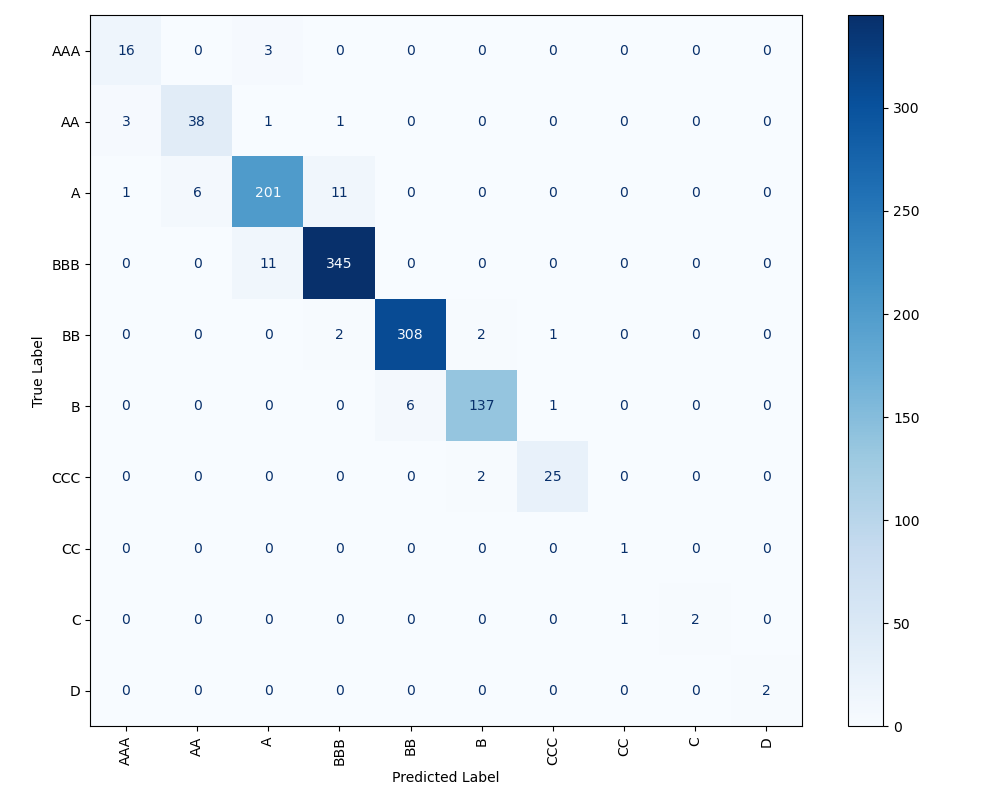
\includegraphics[width=0.6\linewidth,keepaspectratio=true]{../Output/Modelling/Logistic Regression/rating_model_4/rating_model_4_confusion_matrix_no_title.png}
    %     \label{fig:most-complex-confusion-matrix}
	% \end{figure}

    \clearpage
    \newpage

    \subsection{XGBoost - Most Complex Model - Additional Details}

    % Table \ref{tab:most-complex-best-params} and Figure \ref{fig:most-complex-confusion-matrix} show the high level of accuracy we are able to attain even for sparse classes when including all available features with an L1 penalty (elastic net with fully L1), balanced class weighting, and a simple one versus rest multiclass prediction setup (a binary is/is not logistic regression probability is estimated for each class, and class with the highest score is taken).

    % \begin{table*}[h!]
    %     \centering
    %     \caption{Best Hyperparameters - Most Complex Model}
    %     \small
\begin{tabular}{cccccc}
\toprule
C & Class Weighting Strategy & L1 Ratio & Multi-Class Strategy & Penalty & Solver \\
\midrule
0.100000 & Balanced & 1.000000 & One vs Rest & Elastic Net & SAGA \\
\bottomrule
\end{tabular}

\normalsize
    %     \label{tab:most-complex-best-params}
    % \end{table*}

    % \begin{figure}[h!]
	% 	\centering
    %     \caption{Confusion Matrix - Most Complex Model}
    %     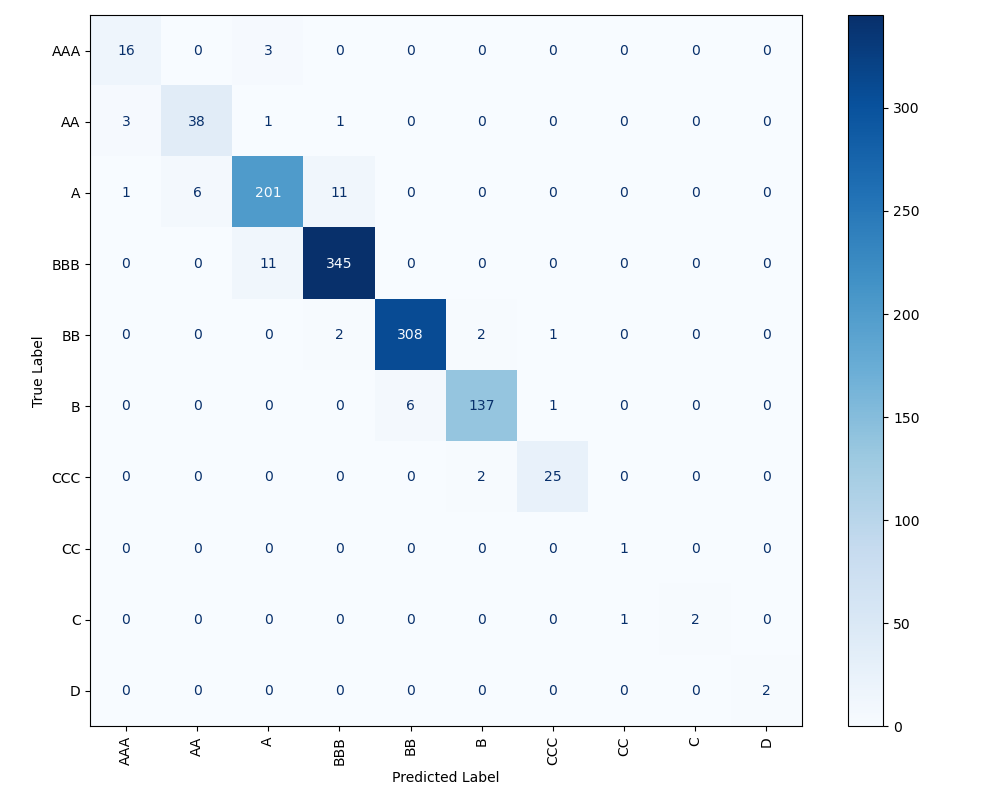
\includegraphics[width=0.6\linewidth,keepaspectratio=true]{../Output/Modelling/Logistic Regression/rating_model_4/rating_model_4_confusion_matrix_no_title.png}
    %     \label{fig:most-complex-confusion-matrix}
	% \end{figure}

    \clearpage
    \newpage

    \subsection{Including Previous Rating}

    \label{sec:include-previous-rating}

    As a reminder, \shareNotChanges \space of ratings remain the same from one fixed quarter date to the next (\shareNotChangesTest \space in our test dataset). Therefore, including rating on the previous fixed quarter date in our predictions leads it to far outweigh the impact of other variables. Table \ref{tab:include-previous-model-comparison} demonstrates our accuracy performance is anchored around the share of ratings that remain the same (with the strange exception of Logistic Regression with Altman Z-Scores only). NLP Features do not add value.

    \begin{table*}[h!]
        \centering
        \caption{Model Comparison Including Previous Rating}
        \begin{minipage}[c]{0.495\linewidth}
            \centering
            \footnotesize
\begin{tabular}{cc}
\toprule
Model/Baseline & Accuracy \\
\midrule
Altman's Z & 0.7442 \\
Financial Variables and Sector & 0.9508 \\
Financial Variables, Sector, and NLP Features & 0.9508 \\
Majority Baseline & 0.3247 \\
\bottomrule
\end{tabular}

\normalsize
            \caption*{\footnotesize Logistic Regression} 
        \end{minipage}
        \begin{minipage}[c]{0.495\linewidth}
            \centering
            \footnotesize
\begin{tabular}{cc}
\toprule
Model/Baseline & Accuracy \\
\midrule
Altman's Z & 0.9517 \\
Financial Variables and Sector & 0.9535 \\
Financial Variables, Sector, and NLP Features & 0.9535 \\
Majority Baseline & 0.3247 \\
\bottomrule
\end{tabular}

\normalsize
            \caption*{\footnotesize XGBoost} 
        \end{minipage}
        \label{tab:include-previous-model-comparison}
    \end{table*}

    Table \ref{tab:include-previous-permutation-importance} substantiates this finding, showing that shuffling previous rating variables leads to a large drop in accuracy. Financial variables round out the list of important contributing features, and contribute far less information.

    \begin{table*}[h!]
        \centering
        \caption{Permutation Importance Including Previous Rating}
        \begin{minipage}[c]{0.495\linewidth}
            \centering
            \tiny
\begin{tabular}{ccc}
\toprule
Permuted Feature & Mean Accuracy Drop & Standard Deviation \\
\midrule
Rating on Previous Fixed Quarter Date BB & 0.256178 & 0.009675 \\
Rating on Previous Fixed Quarter Date BBB & 0.233306 & 0.008979 \\
Rating on Previous Fixed Quarter Date A & 0.111181 & 0.006236 \\
Rating on Previous Fixed Quarter Date B & 0.064464 & 0.003919 \\
Rating on Previous Fixed Quarter Date CCC & 0.013557 & 0.001143 \\
Rating on Previous Fixed Quarter Date AA & 0.010714 & 0.001722 \\
Rating on Previous Fixed Quarter Date D & 0.001829 & 0.000050 \\
Ratio D & 0.000866 & 0.000799 \\
Weighted Average Shares Outstanding (Diluted) & 0.000849 & 0.000249 \\
Other Expenses & 0.000840 & 0.000262 \\
Net Income Ratio & 0.000713 & 0.000779 \\
Numeric Transparency & 0.000703 & 0.000566 \\
EBITDA & 0.000681 & 0.000428 \\
Ratio C & 0.000412 & 0.000538 \\
Ratio B & 0.000130 & 0.000340 \\
\bottomrule
\end{tabular}

\normalsize
            \caption*{\footnotesize Logistic Regression} 
        \end{minipage}
        \begin{minipage}[c]{0.495\linewidth}
            \centering
            \tiny
\begin{tabular}{ccc}
\toprule
Permuted Feature & Mean Accuracy Drop & Standard Deviation \\
\midrule
Rating on Previous Fixed Quarter Date BB & 0.276554 & 0.010192 \\
Rating on Previous Fixed Quarter Date BBB & 0.257352 & 0.010267 \\
Rating on Previous Fixed Quarter Date B & 0.080826 & 0.004940 \\
Rating on Previous Fixed Quarter Date A & 0.047979 & 0.004233 \\
Rating on Previous Fixed Quarter Date AA & 0.036817 & 0.001890 \\
Rating on Previous Fixed Quarter Date CCC & 0.025477 & 0.002348 \\
Rating on Previous Fixed Quarter Date AAA & 0.021269 & 0.002349 \\
Net Property Plant Equipment & 0.001779 & 0.000093 \\
Rating on Previous Fixed Quarter Date C & 0.000900 & 0.000098 \\
Cash Per Share & 0.000834 & 0.000225 \\
Return on Capital Employed & 0.000024 & 0.000150 \\
Market Capitalization & 0.000022 & 0.000140 \\
Operating Cash Flow to Sales & 0.000020 & 0.000131 \\
Cash at Beginning of Period & 0.000000 & 0.000000 \\
Interest Income & 0.000000 & 0.000000 \\
\bottomrule
\end{tabular}

\normalsize
            \caption*{\footnotesize XGBoost} 
        \end{minipage}
        \label{tab:include-previous-permutation-importance}
    \end{table*}

    Previous rating might be available in some real-world prediction scenarios, but absent in others. For predictions for ratings for unrated or entirely new companies or for investors without any rating data, it would not be present, though in standard scenarios concerning movements from quarter to quarter for well-known companies with significant history, it could be.

    \clearpage
    \newpage

    \subsection{Predicting Changes in Rating}

    \label{sec:change-prediction}

    As shown in Figure \ref{fig:credit-ratings}, \shareNotChanges \space of ratings remain the same of ratings remain the same from one fixed quarter date to the next (\shareNotChangesTest \space in our test dataset). This poses a serious challenge for predicting changes, a task easily dominated by the majority class. We implemented SMOTE (Synthetic Minority Over-sampling Technique) \citep{chawla_smote_2002} to oversample the minority classes in the training data and balance the dataset. We also differenced all financial variables that were ratios in order to get useful changes from quarter to quarter (many of our level variables, such as quarterly revenue or income are already quarterly changes in a company's financial position).

    Table \ref{tab:change-model-comparison} shows that SMOTE decreases the accuracy of our models relative to simply predicting the majority class, but increases the recall of the minority classes slightly in some cases (Figure \ref{fig:change-confusion-matrix}). We were not able to find a specification that greatly improved our predictions of minority classes. Improvements in accuracy when adding NLP features are small and insignificant.

    \begin{table*}[h!]
        \centering
        \caption{Rating Changes Model Comparison}
        \begin{minipage}[c]{0.45\linewidth}
            \centering
            \footnotesize
\begin{tabular}{cc}
\toprule
Model/Baseline & Accuracy \\
\midrule
Altman's Z & 0.5742 \\
Financial Variables and Sector & 0.7004 \\
Financial Variables, Sector, and NLP Features & 0.7165 \\
Majority Baseline & 0.9535 \\
\bottomrule
\end{tabular}

\normalsize
            \caption*{\footnotesize Logistic Regression} 
            %\label{tab:most-complex-classification-report}
        \end{minipage}
        \begin{minipage}[c]{0.45\linewidth}
            \centering
            \footnotesize
\begin{tabular}{cc}
\toprule
Model/Baseline & Accuracy \\
\midrule
Altman's Z & 0.8488 \\
Financial Variables and Sector & 0.9454 \\
Financial Variables, Sector, and NLP Features & 0.9490 \\
Majority Baseline & 0.9535 \\
\bottomrule
\end{tabular}

\normalsize
            \caption*{\footnotesize XGBoost} 
            %\label{tab:most-complex-permutation-importance}
        \end{minipage}
        \label{tab:change-model-comparison}
    \end{table*}

    \begin{figure*}[h!]
        \caption{Most Complex Model - Rating Changes Confusion Matrices}
        \begin{subfigure}[h]{0.4925\textwidth}
            \centering
            \subcaption{Logistic Regression}
            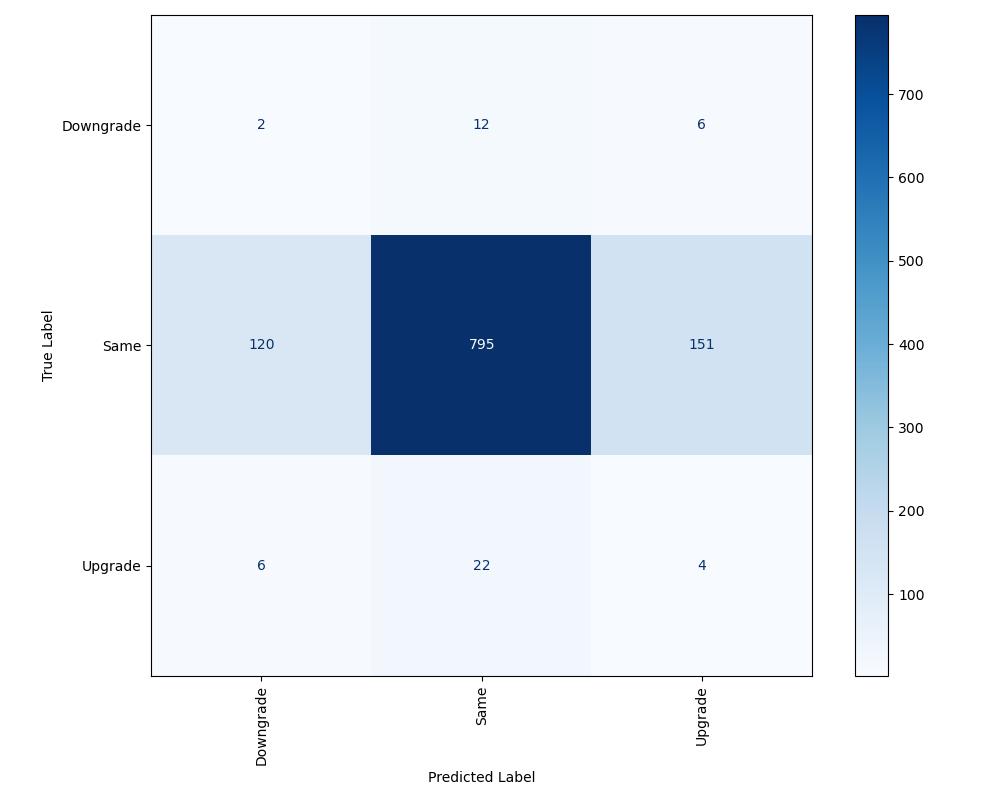
\includegraphics[width=0.95\hsize]{../Output/Modelling/Logistic Regression/smote_rating_change_model_3/smote_rating_change_model_3_confusion_matrix_no_title.png}
        \end{subfigure}
        %\hfill
        \begin{subfigure}[h]{0.4925\textwidth}
            \centering
            \subcaption{XGBoost}
            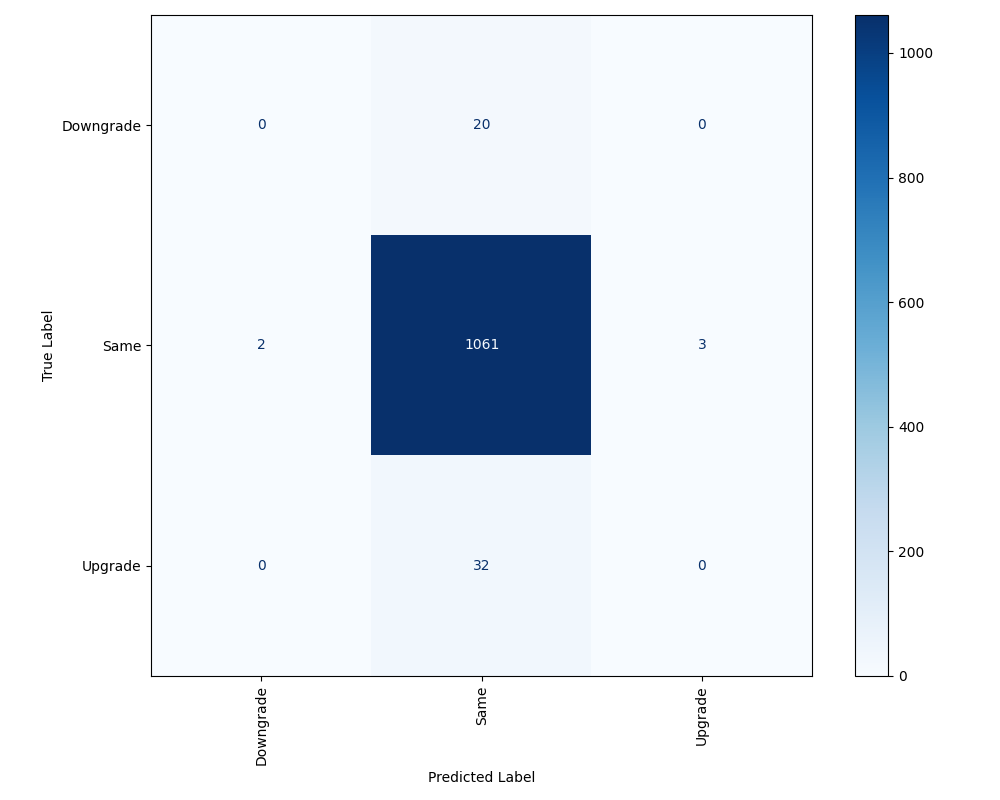
\includegraphics[width=0.95\hsize]{../Output/Modelling/XGBoost/smote_rating_change_model_3/smote_rating_change_model_3_confusion_matrix_no_title.png}
        \end{subfigure}
        \hfill
        \label{fig:change-confusion-matrix}
    \end{figure*}

\end{document}
